\documentclass[conference]{IEEEtran}
% English manuscript, two-platform version (GH200 + MI350X). Replaces main.tex once complete; main.tex keeps the
% GH200-only version until then. Build: tectonic -X compile main_v2.tex
% Figures: gh200/analysis/paper_figures.py and mi350/analysis/paper_figures_mi350.py -> figs/
\usepackage{cite}
\usepackage{amsmath}
% Times-compatible fonts under XeTeX (IEEEtran's ptm Times is not available in the TU encoding tectonic uses)
\usepackage{fontspec}
\setmainfont{texgyretermes}[Extension=.otf,UprightFont=*-regular,BoldFont=*-bold,ItalicFont=*-italic,BoldItalicFont=*-bolditalic]
\setsansfont{texgyreheros}[Extension=.otf,UprightFont=*-regular,BoldFont=*-bold,ItalicFont=*-italic,BoldItalicFont=*-bolditalic]
\setmonofont{texgyrecursor}[Extension=.otf,UprightFont=*-regular,BoldFont=*-bold,ItalicFont=*-italic,BoldItalicFont=*-bolditalic]
\usepackage{unicode-math}
\setmathfont{texgyretermes-math.otf}
\usepackage{graphicx}
\usepackage{booktabs}
\usepackage{multirow}
\usepackage{url}
\usepackage{xcolor}
\usepackage[hidelinks]{hyperref}

\newcommand{\W}{\,W}
\newcommand{\Eh}{\,E$_\mathrm{h}$}
\newcommand{\Ry}{\,Ry}
\newcommand{\ee}[2]{#1{\times}10^{#2}}  % \ee{1.2}{-5} -> 1.2x10^-5 (math mode)
\newcommand{\pct}{\%}
% Results of experiments still running when this draft was written; every occurrence must be gone before submission.
\newcommand{\pending}[1]{\textcolor{red}{[pending: #1]}}

\begin{document}
\bstctlcite{IEEEexample:BSTcontrol}

\title{Unused Mantissa Bits on Power-Capped GPUs: Mechanism, Prediction and Limits on NVIDIA GH200 and AMD MI350X}

\author{\IEEEauthorblockN{Koying Chen}
\IEEEauthorblockA{Department of Computer Science, National Tsing Hua University, Hsinchu, Taiwan}}
% E-mail, co-authors and acknowledgments are left for the author to fill in before submission.

\maketitle

\begin{abstract}
When a GPU runs at its power limit, the energy of every operation sets the clock. We show that zeroing the low-order
mantissa bits an application does not need, in software and on the original FP64, BF16 or FP8 units, turns the
switching power those bits would have spent into throughput, on two vendors' GPUs. On an NVIDIA GH200 cluster and
two 8-GPU AMD MI350X nodes, filling the discarded bits with ones instead of zeros keeps 65--97\pct{} of the saving
across matrix engines, FP64 vector units and memory copies, at three clock settings on MI350X: most of the gain comes
from bits that stop toggling. A two-parameter model built on this mechanism predicts the speedup under any cap from one
calibration within 0.7 (GH200) and 2.0 percentage points (MI350X); on MI350X it must also include a data-dependent
clock reduction that no throttle counter reports. Unlike GH200, MI350X is power-bound at its stock 1000\W{} limit
for FP64, BF16 and FP8 GEMM, so truncation pays at default settings: FP64 HPL keeping 36 significand bits is
4.6\pct{} faster, HPL-MxP keeping 3 bits 4.9\pct{} (7.6 to 8.0\,PFLOP/s per node), a Gaussian-process likelihood
7.6\pct{} and DF-MP2 10.2\pct, rising to 7--20\pct{} at 500\W, with every residual check passed, MP2 energies
within $\ee{2.2}{-8}$\Eh{} and log-likelihoods within $\ee{5}{-8}$ relative; results agree across nodes within 2 points. The limits are equally
clear. INT8 emulation of FP64 beats truncation for large inner dimensions at generous caps, but a tighter cap moves
the crossover toward truncation, because emulation spends its extra integer work at the cap; emulation also needs
workspace that shrinks the solvable problem, and fails silently on data with wide per-row exponent spans. Safe bit
counts are platform-dependent, and chassis fan feedback biases multi-variant interleaved measurements.
\end{abstract}

\begin{IEEEkeywords}
power capping, energy efficiency, floating-point precision, mantissa truncation, GPU, mixed precision, HPL, emulation
\end{IEEEkeywords}

%==================================================================================================
\section{Introduction}

Power is becoming the ceiling on delivered performance. Data centers cap rack power, student cluster competitions
cap the power of a whole cluster, and accelerators ship with board or package limits that their own workloads reach:
the AMD Instinct MI350X holds FP64, BF16 and FP8 matrix multiplication at its default 1000\W{} limit 82--100\pct{} of
the time in our measurements. Under a limit, the power manager lowers the clock until the device fits; the speed of a
program then depends on how much energy each of its operations consumes.

That GPU power depends on input data is known. Bhalachandra et al.\ measured 67\pct{} more power for DGEMM on
random than on constant operands on A100~\cite{Bhalachandra2022}; Gregersen et al.\ varied the distribution and
bit patterns of GEMM inputs and found that zeroing the least significant bits lowers power~\cite{Gregersen2024};
He showed an all-zero matrix multiplication on A100 running about 15\pct{} faster than a random one, with a gap
that widens as the power limit is lowered~\cite{He2024}; Antepara et al.\ measured 563\W{} for a zero-input DGEMM
on GH200 versus 898\W{} for random input~\cite{Antepara2025}; and the TensorRT documentation warns that all-zero
inputs draw less power because fewer DRAM and L2 bits toggle~\cite{TensorRTDocs}. In hardware, Tong et al.\
narrowed floating-point multipliers~\cite{Tong2000}, Pool et al.\ selected precision for graphics
shaders~\cite{Pool2008,Pool2011}, Guenther et al.\ masked mantissas at the inputs of arithmetic
units~\cite{Guenther2016}, and an AMD patent adds a hardware zeroing module to shaders~\cite{AMD2022}.

These works either demonstrate the effect with special inputs such as all-zero or constant data, on one vendor, or
require new hardware or simulated energy. None answers the questions a practitioner faces. Does software truncation of
the low-order mantissa bits of \emph{real} data buy performance on production GPUs of different vendors, and through
which mechanism? Can the gain be predicted before running the application under every cap? How much accuracy does it
cost? And where does it still pay off against format changes such as FP8 or INT8 emulation of
FP64~\cite{Ozaki2025,Uchino2025}, whose own speed also depends on the power limit? To our knowledge this is the first
study that truncates part of the mantissa of real FP64/BF16/FP8 operands in software on production GPUs of two
vendors and measures, on benchmarks and real HPC applications checked by their own correctness criteria, how much
throughput the saved switching power buys under power caps. Our contributions are:

\begin{enumerate}
\item \textbf{The mechanism, across vendors, units and clocks.} Filling the discarded bits with ones or a fixed
pattern instead of zeros separates ``no toggling'' from ``value is zero''. On GH200 and MI350X, in matrix engines,
FP64 vector units and memory copies, at three fixed clocks on MI350X, stopping the bits from toggling captures
65--97\pct{} of the saving with a fill of ones and 41--92\pct{} with a fixed pattern (Section~\ref{sec:why}). On MI350X, truncation also raises the effective clock at a fixed
target clock, a data-dependent clock reduction that no throttle counter reports.
\item \textbf{A predictive model.} If truncation only changes the switched capacitance, the truncated program under
cap $P$ behaves like the native program under $P_0+(P-P_0)/R$. With one calibration it predicts 42 cap--format points
per platform within 0.7 (GH200) and 2.0 percentage points (MI350X, with a clock-stretch term;
Section~\ref{sec:model}).
\item \textbf{Gains on real applications on two platforms.} We express the benefit as the extra cap the unmodified
program needs to catch up, from GEMM to HPL, HPL-MxP, Quantum ESPRESSO, DF-MP2 and a wide-range, power-bound
Gaussian-process likelihood, with paired 95\pct{} intervals, replicated on a second node set on each platform, and check
residuals and energies with each code's own criterion (Section~\ref{sec:results}). On MI350X the gains appear at the
default limit; on GH200 mainly under lowered caps.
\item \textbf{The boundary with format changes.} Against INT8 emulation of FP64 (cuBLAS, GEMMul8) and FP32/3xTF32,
and FP8 for AI, the crossover moves with matrix shape, power cap, memory headroom, accumulation precision and exponent
span; a tighter cap favors truncation on both platforms, and on data with a wide per-row exponent span fixed-width
emulation can silently return wrong results, a risk that a cheap measurement of per-row spans flags beforehand
(Sections~\ref{sec:format}--\ref{sec:ai}).
\item \textbf{Measurement lessons.} Hardware energy accumulators remove the sampling bias of driver power readings;
chassis fans that react to the previous run bias the middle variant of multi-variant interleaved designs; and safe bit
counts must be validated on the target platform (Sections~\ref{sec:setup} and~\ref{sec:hpl}).
\end{enumerate}

Compared with the closest work: Gregersen et al.\ observed input-dependent power and proposed the toggling
hypothesis but avoided throttling and studied only GEMM; He swept the A100 power limit, and Antepara et al.\
measured GH200, but both contrasted all-zero with random inputs without truncating real data or evaluating
accuracy. We quantify the toggling hypothesis on two vendors' module and package power, turn it into a model that
predicts the gain under a cap, show that the data-movement part is consistent with DRAM energy
studies~\cite{Chatterjee2017,Ghose2018}, and quantify speed and accuracy on real applications under caps. Uchino et
al.\ evaluated the speed and energy efficiency of INT8-emulated GEMM~\cite{Uchino2025}; we compare it with truncation
at the same cap and comparable accuracy on two platforms and find that the winner depends on matrix shape and cap.

%==================================================================================================
\section{Background and Related Work}\label{sec:related}

\textbf{Input-dependent GPU power.} Bhalachandra et al.\ argue that power budgets and benchmarks must account for
input entropy~\cite{Bhalachandra2022}. Gregersen et al.\ varied value distribution, bit similarity, ordering and
sparsity of CUTLASS GEMM inputs on A100, H100 and V100 and saw power differ by up to almost 40\pct, with zeroed
low bits lowering power~\cite{Gregersen2024}; they chose sizes that do not throttle, so performance under a cap
was not measured. He reported 295 versus 257\,TFLOP/s for all-zero versus random $8192^3$ GEMMs on A100 and, lowering
the power limit from 330 to 100\W, saw the relative speedup of such predictable inputs grow from about 1.2$\times$ to
about 2.3$\times$ at 150\W{} before it fell at 100\W~\cite{He2024}. Antepara et al.\ measured zero-input DGEMM on
GH200 at 563\W{} and 65.4\,TFLOP/s against 898\W{} and 57.8\,TFLOP/s for random input~\cite{Antepara2025}; their
GH200 roofline study found no significant difference in vector FP64 performance between zero and random
inputs~\cite{Antepara2025W}, consistent with our finding that when the GPU is not power-bound the difference shows
only in power. Ujeniya et al.\ note that constant and random data can differ
by about 100\W{} on H100/H200 but leave it out of scope~\cite{Ujeniya2026}. Lucas and Juurlink built a
data-dependent ALU power model for GTX\,580 whose main term is the number of toggles, with the number of ones a
secondary term~\cite{Lucas2016}. All of these use all-zero, constant or special bit patterns on NVIDIA hardware; none
truncates part of the mantissa of real data, evaluates accuracy or applications, or compares vendors.

\textbf{Power-constrained HPC.} Rountree et al.\ took a first look at performance under a hardware-enforced power
bound and found that manufacturing variation makes nominally identical processors differ by about 6\pct{} in
execution time under the same bound~\cite{Rountree2012}; Inadomi et al.\ measured up to 64\pct{} variation in per-rank DGEMM
performance under a module power cap on a large system and allocated power by variability~\cite{Inadomi2015}.
Patki et al.\ overprovision nodes under a fixed system power budget and enforce per-node bounds~\cite{Patki2013},
and Zeus tunes the GPU power limit together with the batch size to cut DNN training energy~\cite{Zeus2023}. These
works decide how power is distributed; we lower the energy each operation needs, so the two compose. The 13--17\pct{}
node-to-node clock spread we see on GH200 at equal caps, and the 860--1200\,MHz spread among the eight GPUs of one
MI350X node at 800\W{} (Section~\ref{sec:setup}), are consistent with their observations.

\textbf{Hardware mantissa masking and data-movement energy.} Mantissa masking itself is not new. Tong et al.\
showed that many programs tolerate halving the mantissa and that a variable-width multiplier saves up to 66\pct{}
energy per operation~\cite{Tong2000}. Pool et al.\ estimated 23--36\pct{} energy savings in the vertex stage of
mobile GPUs~\cite{Pool2008} and up to 71\pct{} in pixel-shader arithmetic (10--20\pct{} of GPU
energy)~\cite{Pool2011}; Angerd et al.\ automated precision reduction in graphics and designed a register file that
packs arbitrary precisions~\cite{Angerd2017}; Guenther et al.\ masked mantissas at functional-unit inputs of an LTE
baseband processor for up to 23\pct{} energy per task~\cite{Guenther2016}; an AMD patent zeroes mantissa bits in
GPU shaders according to a precision flag~\cite{AMD2022}; and Jahadi and Atoofian exploited the zero bias of
register bits and dropped low-order bits of CNN values to cut tensor-core register-file leakage by
77.3\pct{} in simulation~\cite{Jahadi2024}. rpe and chop use the same bit operations to emulate low precision but
do not measure power~\cite{Dawson2017,Higham2019}. DRAM and HBM energy depend on data toggling
rates~\cite{Chatterjee2017,OConnor2017,Ghose2018}, and compression can reduce bytes but increase
toggles~\cite{Pekhimenko2016}. We differ in being pure software, changing neither hardware nor data format, and in
measuring clocks and performance under caps on production GPUs with validated application accuracy.

\textbf{Precision tuning, mixed precision and power caps.} Tools such as Precimonious lower variable precision for
speed~\cite{RubioGonzalez2013}, and mixed-precision storage reduces bytes per value~\cite{Higham2022}; mantissa
zeroing changes neither type nor bytes and composes with both. Transprecision computing argues for controlling
precision at fine grain in space and time~\cite{Malossi2018}. Closest in form, Grützmacher et al.\ store FP64 values
as mantissa segments that keep the full exponent and read only the leading segments, speeding up memory-bound
PageRank by 10--30\pct~\cite{Grutzmacher2020}; there the truncation saves bandwidth, here switching power.
Low-precision LU with iterative refinement recovers FP64 accuracy~\cite{Haidar2018} and underlies
HPL-MxP~\cite{Dongarra2025}. Klöwer et al.\ estimate from the data itself how many mantissa bits carry real
information and round the rest to nearest to compress atmospheric data~\cite{Klower2021}; the same analysis could
estimate in advance how many bits GEMM operands need, here for power rather than storage. GH200 shares module power
between CPU and GPU and lowers the GPU clock near the cap~\cite{Patrou2025}; Yang et al.\ found that nvidia-smi
samples only about 25\pct{} of runtime on A100/H100~\cite{Yang2024}, which we mitigate on GH200 with long steady
windows, pairing and energy integrated from 1-s averaged power, and avoid on MI350X by reading a hardware energy
accumulator (Section~\ref{sec:setup}).

\textbf{Emulating FP64 on low-precision units.} The Ozaki scheme~\cite{Ozaki2012} splits a matrix product into a sum
of products of lower-precision slices that are computed exactly; Ootomo et al.\ run it on integer matrix
units~\cite{Ootomo2024}, and Ozaki scheme~II uses modular arithmetic~\cite{Ozaki2025} and is implemented in GEMMul8
for CUDA and HIP, with performance and power evaluated by Uchino et al.~\cite{Uchino2025}. cuBLAS ships an
Ozaki-type fixed-point emulation that scales each row of $A$ and column of $B$ by a shared factor, so the dynamic
range within a row is encoded in the mantissa; its automatic mode picks the slice count from the exponent span and
dispatches to native FP64 when more than a library-defined maximum of bits would be needed~\cite{cuBLASEmu,Schwarz2026}.
The benefit of emulation grows with the ratio of INT8 to FP64 throughput, which is about twice as high on MI350X as on
GH200 (Section~\ref{sec:crossover}). These change the arithmetic format; zeroing keeps the original FP64 (or BF16, FP8)
units and lowers input entropy, so the two can be complementary.

\textbf{Mixed precision in geostatistics.} ExaGeoStat evaluates Gaussian-process likelihoods with an FP64 tile
Cholesky~\cite{Abdulah2018}. Its mixed-precision successors order the locations along a space-filling curve so that
strong correlations sit near the diagonal, keep diagonal tiles in FP64 and convert tiles chosen by their distance from
the diagonal or their norm to FP32, FP16 or FP8: 1.6$\times$ on average with FP64/FP32~\cite{Abdulah2019}, up to
2.64$\times$ with FP64/FP32/FP16~\cite{Abdulah2022}, up to 12$\times$ when combined with tile low-rank
compression~\cite{Cao2022}, and 3$\times$ over FP64 on a GH200 with four precisions~\cite{Ren2025}; the same tile method
drove a climate emulator on GH200 systems~\cite{Abdulah2024}. Cao et al.\ also measured the power and energy of such
factorizations on single V100, A100 and H100 GPUs~\cite{Cao2023}, without caps or a clock analysis. Uniform single
precision is insufficient for these likelihoods~\cite{Abdulah2022}, as we also find. All of these convert whole tiles to
another format; we keep FP64 and truncate operand mantissas, and the two compose (Section~\ref{sec:gp}).
Olivares-Amaya et al.\ similarly ran RI-MP2 with single- and mixed-precision GEMMs on GPUs~\cite{OlivaresAmaya2010}.

\textbf{Convergence-driven precision.} Woo et al.\ switch LOBPCG between FP32, FP64 and mixed precision by
convergence state for up to 8.5$\times$ speedup on GPUs~\cite{Woo2023}; Huang, Shao and Hammond choose the number of
INT8 emulation slices in GPU4PySCF from the relative SCF energy change, keeping errors below
$10^{-7}$\,hartree (E$_\mathrm{h}$; 1\,E$_\mathrm{h}$ = 2\,Ry = 627.5\,kcal/mol)~\cite{Huang2026}; Dawson et al.\ found with MPFR that about 37 significant bits suffice for density
matrix purification~\cite{Dawson2024}. All of these gain speed by moving to a higher-throughput format or unit, and
none studies power. We stay on FP64 units, adjust the kept bits one at a time from the Davidson threshold of a
plane-wave code, and gain mainly from clock headroom under a cap (on one of our two test systems also from fewer
Davidson iterations; Section~\ref{sec:adaptive}).

\textbf{FP8 inference and its failures.} FP8 training keeps high-precision master weights with per-tensor
scaling, E4M3 for weights and activations and E5M2 for gradients~\cite{Micikevicius2022}; Gupta et al.\ showed that
rounding decides the fate of low-precision training~\cite{Gupta2015}. The clearest FP8 failure is attention:
FlashAttention-3's FP8 mode drops the VQA-a video-quality score of CogVideoX from 70.2 to 6.5 and of HunyuanVideo from
82.5 to 4.4, and 262k-context retrieval from 7.0 to 0.4, which SageAttention2 repairs inside FP8 by smoothing outliers and using a fixed scale for softmax
probabilities~\cite{Zhang2025}. MLPerf Inference closed division allows any pure, reproducible mathematical
quantization but forbids pruning non-zero weights~\cite{MLPerfInfRules}; mantissa zeroing is the former.

%==================================================================================================
\section{Why Fewer Mantissa Bits Save Power}\label{sec:why}

CMOS dynamic power is roughly $\alpha_\mathrm{sw} C V^2 f$, where the switching activity $\alpha_\mathrm{sw}$ depends
on the data. Under a cap, the power manager lowers $f$ (and $V$) until the device fits, so a lower $\alpha_\mathrm{sw}$
turns directly into higher clock and throughput; below the cap it appears as lower power at the same clock. We see
both on both platforms. On GH200 at the default 1000\W{} module cap, the native FP64 GEMM is still capped 95\pct{} of
the time and runs at 1822\,MHz, whereas keeping 0 bits it runs at the maximum 1980\,MHz while module power falls from
984 to 707\W; under a 700\W{} cap its SM clock is 1502\,MHz native, 1668\,MHz with 27 kept bits and 1965\,MHz with 0
kept bits, all at about 694\W. On MI350X at its default 1000\W{} package power limit (PPT), the native FP64 GEMM is
held at the limit 82\pct{} of the time at 1890\,MHz; with 0 kept bits it never reaches the limit (785\W) and runs at
2183\,MHz, 17\pct{} faster. Native BF16 and FP8 GEMMs are held at the limit 99.8 and 100\pct{} of the time, so every
bit they stop toggling is turned into clock (Table~\ref{tab:fill2}).

\textbf{Toggling or zero?} Zeroing changes two things at once: the low bits stop varying from element to element,
and their value becomes zero. To separate the two we fill the discarded bits with all ones, or with a fixed
nonzero pattern shared by all elements; neither toggles, but neither is zero. On GH200 at 1000\W{} the fills with 0 kept
bits run at the maximum 1980\,MHz (with 20 kept bits at 1963--1971\,MHz, partly capped), so we compare module power;
since the cap holds the native GEMM at 984\W, the share we attribute to ``no toggling'' is conservative. At 500\W{}
every configuration is capped 100\pct{} of the time, so we compare throughput (one node, two runs each). On MI350X we
can do better: we lock the maximum graphics clock at 900, 1300 or 1700\,MHz, below the frequency any configuration
reaches at 1000\W, so that no configuration is power-limited (PPT residency 0--0.6\pct) and the energy per
operation compares switching activity directly (8 GPUs $\times$ ABBA per setting).

\begin{table}[t]
\caption{Share of the zero-fill benefit (\%) that a fill with ones (first number) or a fixed nonzero pattern (second)
retains. GH200: module power at 1000\W{} or throughput at 500\W{} (Section~\ref{sec:why}); MI350X: energy per
operation at a locked clock of 900, 1300 or 1700\,MHz (GEMMs; ranges over the clocks), throughput at 600\W{} or package
power at 1000\W{} (other kernels). Last column: benefit of the zero fill on MI350X (E/op: energy per operation). On
GH200 the zero fill gives 707 versus 984\W{} (FP64, 0 bits), +14.5\pct{} (FP64, 20 bits, 500\W), +28\pct{} (BF16,
500\W), 553 versus 862\W{} (FMA loop) and $-18\pct$ power (copy).}\label{tab:fill2}
\centering\footnotesize\setlength{\tabcolsep}{2.5pt}
\begin{tabular}{@{}lccr@{}}
\toprule
Kernel, kept bits & GH200 & MI350X & MI350X zero fill \\
\midrule
FP64 GEMM, 0 & 76/68 & 73--75/69 & $-20$ to $-29\pct$ E/op \\
FP64 GEMM, 20 (G), 27 (M) & 87/82 & 81--83/73--74 & $-7$ to $-10\pct$ E/op \\
BF16 GEMM, 0 & 92/92 & 77--78/68--72 & $-13$ to $-15\pct$ E/op \\
FP8 GEMM, 0 & --- & 65--66/61 & $-9$ to $-10\pct$ E/op \\
FP64 FMA loop, 0 & 87/62 & 74/63 & +33\pct{} speed \\
Memory copy, 0 & 97/86 & 83/41 & $-9\pct$ power \\
\bottomrule
\end{tabular}
\end{table}

In these measurements merely stopping the low bits from toggling captures most of the benefit, in matrix engines,
FP64 vector units and memory copies of both vendors (Table~\ref{tab:fill2}; ones: 65--97\pct, fixed pattern:
41--92\pct): quantitative support for the toggling hypothesis~\cite{Gregersen2024} beyond one vendor or one unit. On MI350X the shares barely change with the
clock (FP64 with 27 kept bits: 83, 81 and 82\pct{} at 900, 1300 and 1700\,MHz; with 0 kept bits 74, 75 and 73\pct),
while the total saving grows with it (FP64, 0 kept bits: 20, 24 and 29\pct{} less energy per operation), as expected
when the switched-capacitance term $CV^2f$ grows relative to static power. Zeros save somewhat more than ones or a
fixed pattern, and the pattern saves least on the MI350X memory copy (41\pct). With 20--27 kept bits this matches multiplier structure: partial products are $a_i b_j$, so low bits of
$a$ fixed at one still form partial products that toggle with the kept bits of the other operand, whereas zeros keep
that whole slice at zero. With 0 kept bits both mantissas are constant, so the partial products do not toggle under
any fill, yet zeros still save more than ones (GH200: 707 versus 774\W); this may come from simpler alignment and
accumulation of products that are exact powers of two, which we have not verified. We have no gate-level
measurement, so both are inferences consistent with the data. The result also matches the GTX\,580 ALU model of
Lucas and Juurlink, in which toggles dominate and the number of ones in constant inputs is
secondary~\cite{Lucas2016}.

\textbf{Not just matrix engines.} In an FP64 multiply-add loop without matrix units ($8{\times}8$ outer product per
thread), keeping 0 bits lowers GH200 module power at 1000\W{} from 862 to 553\W{} and makes MI350X 16\pct{} faster
at 1000\W{} and 33\pct{} faster at 600\W. In pure memory traffic (a STREAM-like copy) GH200 module power falls by
18\pct{} at 1000\W, and on MI350X, where even a copy is power-bound at 600\W, the copy runs 28\pct{} faster.
Fewer toggles on data wires and in arithmetic units are therefore the main cause, and the effect also exists for
bandwidth-bound code; the data-movement part is consistent with DRAM energy that depends on toggling
rates~\cite{Chatterjee2017,Ghose2018}.

\textbf{A second, invisible clock effect on MI350X.} With the clock locked and no configuration power-limited, the
effective graphics clock still depends on the data. Locked at 1300\,MHz, the native FP64 GEMM runs steadily at
1171--1179\,MHz (5th--95th percentile over 8 GPUs), the same GEMM with 0 kept bits at 1235--1240\,MHz, native BF16 at
1088--1100\,MHz and BF16 with 0 kept bits at 1132--1142\,MHz, at 59--63\,\textdegree C junction temperature. The
power and thermal residency counters read zero, and the firmware's per-XCD ``clock below host limit'' counters stay
at zero even when the power limit is active, so this reduction is reported by none of the counters available to us.
At 1000\W{} without a lock, FP64 with 0 kept bits likewise runs at 2183 rather than 2200\,MHz with no power limiting.
A circuit-level mechanism that stretches the clock when the supply droops under high switching current would explain
these observations; we have no direct measurement of it. Whatever its cause, truncation relieves it too, and the model
of Section~\ref{sec:model} must include it.

%==================================================================================================
\section{A Model of Truncation Gains Under a Power Cap}\label{sec:model}

Let a GPU under cap $P$ settle at a target clock $f$ with $P = P_0 + c\,g(f)$, where $P_0$ is the power that does
not scale with switching (static and uncore), $g(f) = V(f)^2 f$ is the voltage--frequency curve of the device, shared
by all programs, and $c$ is the program's effective switched capacitance. Truncation changes only $c$. Let the effective
clock be $s\,f$, where $s\le1$ is the clock reduction of Section~\ref{sec:why} (MI350X) and performance is
proportional to the effective clock. Write $\sigma = s_r/s_n$ for the ratio of effective clocks of the truncated
($r$) and native ($n$) programs and $R = (c_r s_r)/(c_n s_n)$ for the ratio of their dynamic powers, both measured at
one locked clock. Then the truncated program under cap $P$ reaches the clock the native program reaches under
\begin{equation}
P' = P_0 + (P - P_0)/R,
\end{equation}
and its performance is
\begin{equation}
p_r(P) = \sigma\,p_n(P'), \qquad \Delta W = P' - P = (P-P_0)\left(\tfrac{1}{R}-1\right),
\end{equation}
capped at the program's clock-limited peak. The equivalent power saving is thus proportional to the dynamic part of
the cap, and the whole curve follows from the native curve $p_n(P)$ and two numbers measured once.

We test two calibrations. (a)~\emph{Fixed clock} (MI350X): $R$ and $\sigma$ from the locked-clock runs of
Section~\ref{sec:why} at 1300\,MHz, with $P_0$ fitted once per platform. (b)~\emph{One cap} (both platforms):
$\sigma=1$ and $R$ from the measured speed at the lowest cap only. Predictions are compared with the measured speedups
of the GEMM sweeps at the other caps (GH200: 300--1000\W, 6 points per format; MI350X: 400--1000\W, 7 points, node
n02).

\begin{figure}[t]
\centering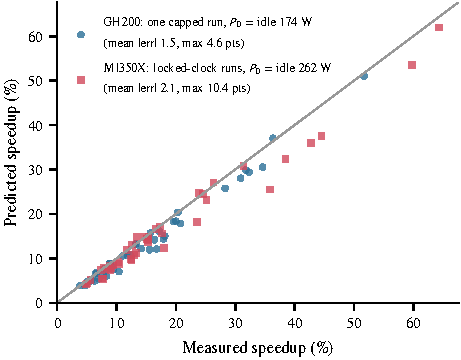
\includegraphics[width=\columnwidth]{figs/mi350_model.pdf}
\caption{Predicted against measured GEMM speedups under caps for FP64 (0, 12/27, 35/36 kept fraction bits), BF16 (0, 3)
and FP8 (0). GH200: calibrated at the lowest cap (that point excluded); MI350X: from locked-clock power and clock
alone. MAE: mean absolute error in percentage points.}\label{fig:model}
\end{figure}

The model predicts both platforms well (Fig.~\ref{fig:model}). On GH200 the one-cap calibration predicts the other 42
points within 0.7 percentage points on average (largest error 2.7) with $P_0=200$\W. On MI350X the fixed-clock
calibration, which uses no point of the cap sweep, predicts the 42 points within 2.0 points on average with
$P_0=250$\W{}, which matches the measured idle power of 244--264\W{} per GPU; without the clock-stretch term the error
is 2.5 points, and with $P_0=0$, i.e., if all power were dynamic, it is 4.0. The ratios are $R=0.94$, 0.89 and 0.67 for
FP64 with 36, 27 and 0 kept bits, 0.92 and 0.85 for BF16 with 3 and 0 bits and 0.90 for FP8 with 0 bits, with
$\sigma=1.010$--1.053. The residual errors concentrate where the model's assumptions break: FP64 with 0 kept bits at
500--800\W{} is underpredicted by 6--7 points, as its clock rises into the range where the native curve is not
measured (the native FP64 GEMM never exceeds 1890\,MHz, the truncated one reaches 2180\,MHz), and BF16 at 400\W, where
the native GEMM barely runs, by 5--9 points. For the bit counts that applications use (FP64 with 27--36 bits, BF16
with 3 bits, FP8) the error is at most 3 points. The practical consequence is that a single locked-clock measurement of
the truncated kernel, or a single run at one cap, predicts its benefit under every cap; and $\Delta W\propto P-P_0$
explains why the equivalent saving grows with the cap even where the relative speedup does not.

%==================================================================================================
\section{Method}\label{sec:method}

\textbf{Mantissa zeroing.} For a floating-point operand with $p$ fraction bits (52 for FP64, 7 for BF16, 3 for FP8
E4M3) we keep the top $k$ fraction bits and set the remaining $p-k$ to zero. Sign and exponent are untouched, so
the representable range is the format's full range. We compare truncation toward zero (one bit mask),
round-to-nearest (add half a unit of the last kept bit, then mask) and stochastic rounding (add a uniform random
integer below the weight of the discarded bits, then mask). Ties go away from zero in the shim, the GEMM
microbenchmark, Quantum ESPRESSO, DF-MP2 and the Gaussian-process code, and to even in HPL, the LoRA weight loading
and LLM inference. We write ``truncate to $k$ bits'' for keeping $k$ bits either way: unless stated otherwise, the
applications (Quantum ESPRESSO, PySCF, DF-MP2, Gaussian process, ExaGeoStat, third-party codes) and HPL round to
nearest, while the GEMM microbenchmarks and HPL-MxP truncate toward zero, and the crossover sweeps of both platforms
round to nearest on MI350X and truncate on GH200. HPL counts significand bits including the hidden bit, as rocHPL does:
its 36 bits are 35 fraction bits. Each element costs one integer AND (plus an add for rounding), which can be fused into
the kernel that produces the operand; here HPL runs a separate rounding kernel and the shim makes a copy, and both costs
are included in the measured times.

\textbf{Error model.} For operands uniform on $[-1,1)$ with both $A$ and $B$ zeroed, the relative error of $C=AB$ is
\begin{equation}
\lVert \hat C - C\rVert_F \,/\, \lVert C\rVert_F \approx \alpha\,2^{-k},
\end{equation}
with $\alpha\approx0.27$ for round-to-nearest, 0.38 for stochastic rounding and 0.70 for truncation ($k\ge4$;
truncation errs about 2.6 times more than round-to-nearest), independent of the inner dimension from 256 to 16384
(measured by splitting the error terms exactly in FP64). Truncation's error is almost entirely a systematic
shrinkage: the least-squares slope of $\hat C$ against $C$
departs from 1 by about $-0.6\cdot 2^{-k}$ ($-0.59$ to $-0.64$ across $k$). This matters little for solvers that
iterate to self-consistency or correct with a residual, but hurts processes that accumulate bias, which is why the
rounding mode matters so much in Sections~\ref{sec:results}--\ref{sec:ai}. The relative errors measured on MI350X
($\ee{7.8}{-12}$ at 35 bits and $\ee{2.0}{-9}$ at 27 bits, nearest) agree with the model.

On real Llama2-70B layer-40 activations and weights, $\alpha=0.22$ (nearest) and 0.66--0.68 (truncation) for
$k=2$--4, within about 20\pct{} of uniform data. On four real FP64 GEMMs of Quantum ESPRESSO Si\,1000, $\alpha$ is
0.19--0.32 (nearest) and 0.72--0.81 (truncation). On four real GEMMs of a gold surface, $\alpha$ is nearly constant
across $k$ within each GEMM, confirming the $2^{-k}$ law, but ranges from 0.07 to 9.6 (nearest) across GEMMs
with the amount of cancellation: for nearly orthogonal overlaps such as $\langle\psi|\psi\rangle$ the result norm is
far below the product of operand norms, amplifying the relative error. The form of the model holds broadly, but the
prefactor must be measured per application; self-consistent iteration corrects these errors, which is why Quantum
ESPRESSO tolerates 20--28 bits even with $\alpha\approx 10$.

\textbf{Equivalent power saving.} Under cap $P$, let the zeroed program reach performance $p'(P)$. Its equivalent
power saving is
\begin{equation}
\Delta W(P) = P_\mathrm{native}\bigl(p'(P)\bigr) - P,
\end{equation}
where $P_\mathrm{native}(x)$ is the cap at which the native program reaches performance $x$, linearly interpolated
along the measured performance--cap curve. $\Delta W$ is the extra power budget per node (GH200) or per GPU (MI350X)
the unmodified program needs to match the zeroed one. If $p'$ exceeds every native point we report a lower bound; if
the GPU is not power-bound, the saving appears as lower measured power at the same speed. Because performance is
concave in the cap, linear interpolation between widely spaced caps (e.g., 800 and 1000\W) slightly overestimates
$\Delta W$. Section~\ref{sec:model} gives a closed form.

\textbf{Tolerance-driven precision.} Many solvers tighten their tolerance as they converge. In plane-wave DFT each
Davidson diagonalization receives a threshold $\mathit{ethr}$ that tightens from about $10^{-2}$ to about $10^{-13}$
during the self-consistent-field (SCF) iteration. We keep
\begin{equation}
k = \mathrm{clamp}\bigl(\lceil -\log_2 \mathit{ethr}\rceil + m,\ k_{\min},\ 52\bigr)
\end{equation}
fraction bits (margin $m$, floor $k_{\min}=16$), so early iterations use fewer bits and the last ones use what the
tolerance requires. This is an empirical rule, not a guarantee: $\mathit{ethr}$ is an absolute eigenvalue tolerance
(in Ry), not a relative mantissa error, and the margin absorbs the difference. It needs no application model, only
a tolerance the application already computes.

%==================================================================================================
\section{Experimental Setup}\label{sec:setup}

\textbf{GH200 system.} Fourteen nodes, each with one NVIDIA GH200 480GB superchip (72-core Neoverse-V2 Grace; Hopper
GPU with 96\,GB HBM3, maximum SM clock 1980\,MHz, FP64 tensor-core peak 67\,TFLOP/s~\cite{NVIDIAGH200}), connected by
200\,Gb/s InfiniBand and managed by Slurm. The module power cap covers GPU, CPU and memory; the driver accepts caps
from 200 to 1000\W{} (default 1000\W), while the datasheet lists 450--1000\W~\cite{NVIDIAGH200}, so our caps below
450\W{} lie outside that range (measured power still follows them). The GPU alone has a separate 900\W{} limit.
The default of 1000\W{} is also the highest cap, not an uncapped state: native HPL and FP64 GEMM still hit it much of
the time. Software: NVHPC 26.5 (CUDA 13.2, cuBLAS 13.4, NCCL 2.29, HPC-X Open MPI 5), driver 615.71.

\textbf{MI350X system.} Two nodes, each with eight AMD Instinct MI350X OAM GPUs (gfx950, 256 compute units, 288\,GB
HBM3E, maximum graphics clock 2200\,MHz) connected by Infinity Fabric, Ubuntu 24.04, ROCm 7.2.3 (rocBLAS, hipBLASLt,
RCCL), Open MPI 5.0.7 with UCX, managed by Slurm. The package power limit (PPT0) per GPU is set with \texttt{amd-smi}
from 1 to 1000\W; the default of 1000\W{} is the maximum. We use 400--1000\W. Idle power is 244--264\W{} per GPU,
so a 500\W{} cap leaves about half the dynamic budget.

\textbf{Workloads.} (1)~GEMM microbenchmarks with cuBLAS (GH200) and rocBLAS/hipBLASLt (MI350X): FP64
$32768{\times}32768{\times}2048$; BF16 and FP8 E4M3 $32768{\times}32768{\times}k$ ($k=6144$ on GH200, 8192 on MI350X) with
FP32 accumulation, on operands uniform on $[-1,1)$. (2)~HPL and HPL-MxP. On GH200: a CUDA port of rocHPL, FP64, 8 nodes,
tuned to $N=286720$, NB 1024, a $2\times4$ grid, split fraction 0.05 and NCCL fixed at 8 channels with 2\,MiB buffers;
HPL-MxP (BF16 LU, FP32 accumulation, FP64 iterative refinement, 8 nodes, $N=491520$, on a diagonally dominant test
matrix). On MI350X, one node of 8 GPUs: rocHPL ($N=540672$, NB 1024, $1\times8$, split fraction 0.1, the best
native configuration we found earlier) and the same HPL-MxP code ($N=1034752$, NB 5504, $4\times2$, 7.6\,PFLOP/s native).
(3)~Quantum ESPRESSO 7.6 GPU~\cite{Giannozzi2020} (Si 1000-atom supercell at $\Gamma$, DGEMM; Au 112-atom surface with
$k$ points, ZGEMM), GPU4PySCF 1.8.1~\cite{Wu2025,Li2025} (valinomycin B3LYP/def2-TZVP with density fitting; taxol RHF and
DF-MP2) and three non-GEMM FP64 codes (MFEM, SW4, LAMMPS) on GH200; DF-MP2 on MI350X with the three-index tensor of
the same taxol calculation built by PySCF 2.14 on the CPU and the contraction on the GPU (GPU4PySCF does not support
ROCm; the correlation energy matches PySCF's to $\ee{2}{-13}$\Eh{} and GPU4PySCF's on GH200 to $\ee{7.5}{-8}$\Eh); and a
Gaussian-process likelihood on both (Section~\ref{sec:gp}). (4)~MLPerf Training Llama\,2 70B LoRA with NVIDIA's v5.0
implementation (FP8 weights and GEMMs, activations offloaded to Grace memory), 8 GH200 nodes, global batch 8, and
inference on six language models.

\textbf{Implementation.} Microbenchmarks and HPL-MxP zero operands in the kernel that produces them; HPL rounds both
operands in a separate kernel before each FP64 DGEMM. For unmodified scientific software on GH200 an
\texttt{LD\_PRELOAD} shim intercepts cuBLAS DGEMM/ZGEMM, GemmEx and strided-batched calls and CPU dgemm/zgemm, writes
zeroed copies of $A$ and $B$ to scratch buffers (the caller's data are unchanged) and can record exponent histograms
and per-row exponent spans of the operands. Quantum ESPRESSO is additionally modified to zero the Davidson vectors in
place; DF-MP2 and the Gaussian-process code zero their operands in place; LoRA zeroes the frozen FP8 base weights once
after loading. GEMMul8~3.2.0 (MI350X) and cuBLAS emulation (GH200) replace FP64 GEMMs through a hook or the cuBLAS math
mode. Table~\ref{tab:settings} lists what the bit count means, how bits are removed and how many samples each experiment
has.

\begin{table}[t]
\caption{Bit counts, rounding and samples per experiment (G: GH200, M: MI350X).}\label{tab:settings}
\centering\footnotesize\setlength{\tabcolsep}{2.5pt}
\begin{tabular}{@{}p{0.29\columnwidth}p{0.2\columnwidth}p{0.18\columnwidth}p{0.27\columnwidth}@{}}
\toprule
Experiment & Bits $k$ & Removal & Samples \\
\midrule
GEMM, fill controls, crossover & fraction bits & G: trunc.; M: trunc.\ (crossover: nearest) & G: 3 nodes $\times$ 2 pairs; M: 8 GPUs $\times$ 2 pairs, 2 nodes \\
HPL & significand bits (36 = 35 fraction) & nearest, ties to even & G: 2 node sets, 6 pairs; M: 2 nodes, 2--4 pairs \\
HPL-MxP & BF16 fraction bits & truncation & G: 2 node sets, 6 pairs; M: 2 nodes, 4 pairs each \\
QE, PySCF, DF-MP2, Gaussian process, ExaGeoStat, MFEM, SW4, LAMMPS & fraction bits & nearest, ties away & G: QE warm-up + 6 pairs; DF-MP2, GP 6 rounds; M: DF-MP2, GP 16 per cap \\
LoRA & FP8 fraction bits & truncation (also nearest, stochastic) & G: 2 seeds, 4 pairs \\
LLM inference & BF16/FP8 fraction bits & nearest, ties to even & G: 6 models \\
\bottomrule
\end{tabular}
\end{table}

\textbf{Measurement protocol.} On GH200, nvidia-smi samples power, SM clock, temperature and throttle reasons every
250--500\,ms; on MI350X a sampler reads the GPU metrics table of all eight GPUs every 100\,ms (4\,ms per sweep):
package power, the clock of each of the eight XCDs, temperatures, the cap in effect, and two hardware accumulators, a
15.26-$\mu$J energy counter and the residency of power and thermal limiting. Energy on MI350X is the difference of the
energy counter across a window, which agrees with the mean sampled power to within 0.1\pct{} over long windows. Every
measurement starts from a cooled GPU (GH200: below 45\,\textdegree C; MI350X: junction below 63\,\textdegree C, with at
least 60\,s of rest in the paired designs below); within a cap the variants run in ABBA order on the same GPUs. On
MI350X all eight GPUs run the same configuration at once, so each window yields eight paired samples. Each sample
records the cap actually in effect, and windows whose cap differs from the intended one are discarded (another user's
tool reset caps on the GH200 cluster at least twice; the affected measurements were rerun). Hardware power-brake
events on GH200 are read from cumulative throttle counters. The first native run of a job is often slower (warm-up),
and since ABBA sequences usually start with native, the first pair can overstate the gain (Section~\ref{sec:adaptive}),
so the repeat runs start with one uncounted warm-up run. MLPerf comparisons always use the same seed, i.e., the same
data order.

\textbf{A pitfall: chassis fans and multi-variant interleaving.} On MI350X at 800\W, a three-variant ABBA sequence of
HPL-MxP (native, 4 bits, 3 bits, then reversed) made the 4-bit variant look faster than the 3-bit one, opposite to
the second node and to the phase profile. The node's temperature trace shows why: after a hot run the chassis fans
speed up, the junction temperature falls by 25\,\textdegree C within 20\,s, the cool-down condition is met at once and
the next run starts under high airflow and stays about 12\,\textdegree C cooler; the run after it, under relaxed fans,
is hot again. The middle variant of a three-variant sequence always follows a hot run, so it was systematically
cooler and its slowest GPU ran 20--30\,MHz faster. No such position effect appears at the other caps (mean temperature
differences by position $\le1.5$\,\textdegree C), and two-variant ABBA blocks are immune because each variant takes each
position equally often. We therefore rerun all multi-variant comparisons as pairwise ABBA blocks (reference $v$ $v$
reference) with a minimum rest, and report the affected cell separately (Section~\ref{sec:hpl}).

\textbf{Power, energy and statistics.} On GH200, energy integrates the driver's 1-s averaged module power over the
measurement window, summed over nodes. Power in watts in tables and text is the mean of the instantaneous samples in a
steady window; over 845 steady windows it agrees with the 1-s average within $\pm0.6\pct$, but on bursty kernels (e.g.,
cuBLAS FP64 emulation) single instantaneous readings deviate by $-37\pct$ to $+41\pct$, so energy does not use them.
While the cap is hit, the 1-s average is often below the cap, so the limiter acts on a shorter, unknown time scale.
Module power includes GPU, CPU and memory; under GEMM load the GPU accounts for 88--90\pct{} of it at 900--1000\W,
falling to 77\pct{} at 400\W. On MI350X power is per GPU package and includes its HBM. Confidence intervals use paired
differences: each ``zeroed\,/\,native$\,-\,1$'' on the same node (GPU), cap and ABBA round is one sample, and we report
95\pct{} $t$ intervals, which removes the node-to-node and GPU-to-GPU clock spread. The intervals treat pairs from one job
or node as independent, which they are not fully, so they may be too narrow; for this reason every MI350X result was
repeated on the second node.

%==================================================================================================
\section{Results: Gains Under Power Caps}\label{sec:results}
\subsection{GEMM}\label{sec:gemm}

\begin{figure*}[t]
\centering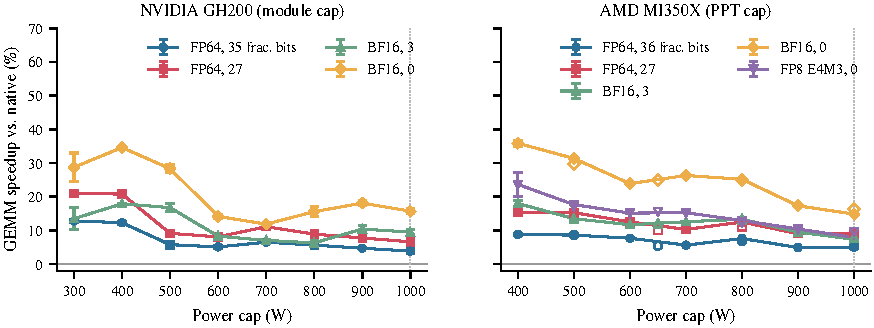
\includegraphics[width=\textwidth]{figs/mi350_gemm_caps.pdf}
\caption{GEMM speedup from mantissa zeroing under power caps on GH200 (module cap; FP64
$32768{\times}32768{\times}2048$, BF16 $k=6144$; 3 nodes $\times$ ABBA) and MI350X (package cap; BF16 and FP8
$k=8192$; 8 GPUs $\times$ ABBA on node n02). Bars: 95\pct{} paired intervals. The dotted line marks each platform's
default limit, which is also its highest.}\label{fig:gemm}
\end{figure*}

Zeroing speeds up GEMM at every cap on both platforms, but the gain does not grow monotonically as the cap tightens
(Fig.~\ref{fig:gemm}). On GH200, FP64 keeping 27 bits is $9.1\pm1.0$, $8.1\pm0.2$, $11.1\pm0.3$ and $8.9\pm1.0\pct$
faster at 500, 600, 700 and 800\W{} (95\pct{} intervals, 6 paired samples per point), an equivalent saving $\Delta W$ of
79--162\W; BF16 keeping 0 bits is 11.9--28.3\pct{} faster, $\Delta W$ from 121\W{} to above 200\W. On MI350X the
default limit already binds, so the gains start there: at 1000\W{} FP64 keeping 36, 27 and 0 bits is 5.0, 9.1 and
16.7\pct{} faster, BF16 keeping 3 and 0 bits 7.4 and 14.8\pct, and FP8 E4M3 keeping 0 bits 7.9\pct{} (node n02;
node n01, 16 pairs per point: 5.2, 9.3, 17.3, 7.9, 16.4 and 9.6\pct{} with intervals of $\pm$0.2--1.3 points). Toward
400\W{} the gains grow to 8.9, 15.5 and 65\pct{} (FP64), 19.1 and 38.5\pct{} (BF16) and 28.2\pct{} (FP8), and the equivalent
saving per GPU is 42--72\W{} for FP64 with 36 bits at 600--900\W{} and 73--147\W{} for BF16 with 0 bits at 600--800\W. The two MI350X
nodes agree within 1.8 points at every common cap and format. The most energy-efficient cap shifts with truncation:
on GH200 native FP64 peaks at 82\,GFLOP/J at 500\W{} and FP64 keeping 27 bits at 90\,GFLOP/J at 400\W, native BF16
at 950\,GFLOP/J at 600\W{} and BF16 keeping 0 bits at 1159\,GFLOP/J at 500\W; on MI350X native FP64 peaks at
63\,GFLOP/J at 700\W{} and FP64 keeping 36 bits at 68\,GFLOP/J at 800\W, native BF16 at 988\,GFLOP/J at
900--1000\W{} and BF16 keeping 0 bits at 1169\,GFLOP/J at 800\W.

Against quantizing to FP8 (GH200, 575\W, relative to native BF16), BF16 zeroed to 0 bits gives 1.15$\times$, native FP8
E4M3 1.87$\times$ and FP8 zeroed to 0 bits 2.12$\times$. On uniform data FP8 E4M3 errs by 3.6\pct, close to
BF16 truncated to 4 bits (4.35\pct) or rounded to nearest at 3 bits (3.34\pct). On narrow-range data, including
the real Llama\,2 70B weights, FP8 wins in both speed and accuracy. On data whose rows span $2^{-24}$ to $2^{24}$,
however, FP8 flushes 63\pct{} of the values to zero (median elementwise error 100\pct) while the Frobenius error is
only 3.9\pct; BF16 keeps every value's magnitude even at 0 bits.

\subsection{HPL and HPL-MxP}\label{sec:hpl}

\begin{table}[t]
\caption{HPL scaled residuals (threshold 16; repeated runs reproduce exactly). Bits are significand bits including
the hidden bit (36 bits = 35 fraction bits), rounded to nearest even. GH200: 8 nodes at 1000\W, $N=286720$ is the tuned
configuration of the cap sweep; MI350X: one node of 8 GPUs at 1000\W. (F): fails the check; bold: the failures that
rule out 28 bits.}\label{tab:hpl}
\centering\footnotesize\setlength{\tabcolsep}{3pt}
\begin{tabular}{@{}lrrrrrr@{}}
\toprule
$N$ & Native & 36 bits & 32 bits & 30 bits & 28 bits & 24 bits \\
\midrule
\multicolumn{7}{@{}l}{\emph{GH200}} \\
131072 & $\ee{1.5}{-4}$ & 0.16 & --- & --- & 13.97 & 456 (F) \\
196608 & $\ee{1.3}{-4}$ & 0.072 & --- & --- & \textbf{18.09 (F)} & 462 (F) \\
262144 & $\ee{2.6}{-5}$ & 0.042 & --- & --- & 14.70 & 91 (F) \\
286720 & $\ee{7.6}{-5}$ & 0.038 & --- & --- & 15.40 & --- \\
\multicolumn{7}{@{}l}{\emph{MI350X}} \\
262144 & $\ee{5.4}{-5}$ & 0.46 & 11.1 & 84 (F) & \textbf{514 (F)} & --- \\
393216 & $\ee{4.6}{-5}$ & 0.15 & 12.0 & 20.2 (F) & \textbf{104 (F)} & --- \\
540672 & $\ee{7.8}{-6}$ & 0.27 & 3.5 & 17.3 (F) & \textbf{102 (F)} & --- \\
\bottomrule
\end{tabular}
\end{table}

The HPL residual check determines the usable bit count, it must be checked at several sizes, and the answer depends
on the platform (Table~\ref{tab:hpl}). On GH200, from 36 to 28 bits the residual grows 86--410$\times$, of the order of
$2^8=256$, so 28 bits sits less than one bit from the threshold and is not an operating point, whereas 36 bits leaves
a margin of about 100$\times$ (at least 98$\times$, about seven bits). On MI350X the same 28 bits fails at every size we
tried, by 6--32$\times$, and even 30 bits fails; 32 bits passes with a margin of only 1.3--4.6$\times$, and 36 bits passes
with 35--100$\times$. The two platforms run different HPL builds and BLAS libraries (blocking and accumulation order of
rocBLAS and cuBLAS DGEMM differ), so a bit count validated on one system does not transfer; 36 bits is safe on both.

\textbf{GH200, 8 nodes.} We first tuned native HPL at 1000\W. The configuration inherited from an H200 study ($N=262144$, NB 1024,
$2\times4$, default NCCL) gave 374.8--376.0\,TFLOP/s; fixing NCCL at 8 channels with 2\,MiB buffers (+4.5\pct) and
raising $N$ to 286720 (+2\pct) gave 390.2--398.8\,TFLOP/s in three runs, and no neighboring setting of $N$, NB, split
fraction or NCCL parameters beat this ${\approx}2\pct$ run-to-run spread (24 settings, 26 runs; $f=0.15$ and
$4\times2$ grids were about 2 and 13\pct{} slower). We then swept the caps with this configuration on two node sets: set
A (work4--11) with two ABBA pairs per cap, and set B (work3--8, 12 and 13), measured a day later after one uncounted
warm-up run, with four pairs per cap. That day the second InfiniBand port of most nodes linked at only 2.5\,Gb/s and
NCCL and MPI routed part of the traffic over it (157\,TFLOP/s on 8 nodes); pinned to the 200\,Gb/s port, set B still
reached only 365.5\,TFLOP/s natively at 1000\W, 7\pct{} below set A, although its SM clock was higher (1961 versus
1936\,MHz), so more of its time went to communication. Differences between the sets thus mix nodes and network state; every
pair is matched within one job.

With 36 bits, GH200 HPL is 3.3--4.7\pct{} faster at 500--800\W{} over the 6 pairs (95\pct{} intervals of $\pm$0.1--0.5
points; set A 4.0--5.0\pct, set B 3.0--4.6\pct; Table~\ref{tab:hplperf}, Fig.~\ref{fig:hpl}), uses 4.1--4.6\pct{} less
energy per solve, and is worth $\Delta W=42$--74\W{} per node at 500--700\W{} (at 800\W{} the interpolation across the
800--1000\W{} gap overestimates). The speedups stay below the SM clock gains (4.5--7.0\pct), consistent with
communication time that does not shrink with the clock, and set B, which communicates longer, gains less. Pairs within
a job agree to within 0.4 (set B) and 0.6 points (set A), but the sets differ by up to 0.9 points at 600--800\W, so two
pairs on one node set understate the uncertainty, and the pooled interval, which treats the 6 pairs as independent,
may still be too narrow. At 400\W, below the specified range, the gain is $9.9\pm1.0\pct$ (sets A/B: 11.0/9.3\pct)
against only 6.3--6.6\pct{} more SM clock, for reasons we have not identified. At the default 1000\W{} cap both sets
use less energy per solve (7.5/8.6\pct; pooled $8.3\pm1.1\pct$), but the speedup depends on how far the cap pulls the
native clock down: native set A is capped in 75\pct{} of the samples at 1936\,MHz and also thermally throttled in
15\pct{} of them (36 bits: 5\pct; no other cap or set throttles), and the 36-bit run is 3.9\pct{}
faster, partly a temperature effect, whereas native set B averages 1961\,MHz, 1\pct{} below the maximum, and gains only 0.6\pct. Tuned native HPL
reaches 393.9\,TFLOP/s at 1000\W{} on set A (mean of two runs; 398.8\,TFLOP/s at best during tuning), about 73\pct{} of
the 8 GPUs' FP64 tensor-core peak, and the 36-bit run 409.2\,TFLOP/s (research results, not official scores). The
untuned configuration gave 3.4--8.3\pct{} at 400--800\W{} and 0.7/7.7\pct{} at 1000\W. (On set A, 28 bits is
5.7--16.3\pct{} faster at 400--800\W, but its residual reaches 15.4 at $N=286720$; we list it only as a boundary
reference.)

\begin{figure}[t]
\centering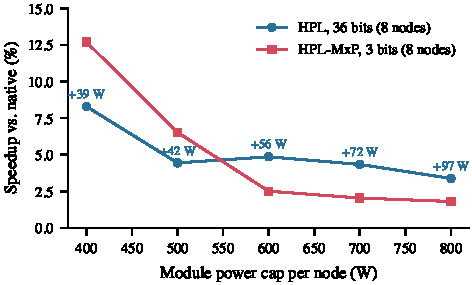
\includegraphics[width=\columnwidth]{figs/hpl_caps.pdf}
\caption{GH200: 8-node HPL (36 significand bits, tuned, $N=286720$) and HPL-MxP (3 kept bits, $N=491520$, diagonally dominant
test matrix) speedups: mean $\pm$ 95\pct{} $t$ interval over 6 pairs from two node sets; open markers are each set's
mean.}\label{fig:hpl}
\end{figure}

\begin{table}[t]
\caption{GH200: delivered performance on 8 nodes in TFLOP/s, node set A\,/\,B (means per set). HPL: tuned, $N=286720$;
HPL-MxP: $N=491520$, reportable rate including refinement. The 8 GPUs' FP64 tensor-core peak is about 536\,TFLOP/s
($8\times67$\,TFLOP/s~\cite{NVIDIAGH200}).}\label{tab:hplperf}
\centering\footnotesize\setlength{\tabcolsep}{3pt}
\begin{tabular}{@{}lcccc@{}}
\toprule
& \multicolumn{2}{c}{HPL (FP64)} & \multicolumn{2}{c}{HPL-MxP (BF16 LU)} \\
\cmidrule(lr){2-3}\cmidrule(l){4-5}
Cap & Native & 36 bits & Native & 3 bits \\
\midrule
400\W & 225.0/228.0 & 249.9/249.2 & 2076/1922 & 2340/2128 \\
500\W & 288.0/278.2 & 300.7/291.0 & 2823/2555 & 3007/2692 \\
600\W & 318.0/304.5 & 334.0/318.3 & 3229/2858 & 3310/2922 \\
700\W & 346.2/328.3 & 362.9/341.3 & 3449/3039 & 3519/3094 \\
800\W & 370.8/345.8 & 385.6/356.3 & 3655/3178 & 3720/3229 \\
1000\W & 393.9/365.5 & 409.2/367.5 & ---$^{*}$ & --- \\
\bottomrule
\end{tabular}
\\[2pt]{\scriptsize Set A: work4--11 (HPL), work4--7 and 10--13 (HPL-MxP), 2 pairs per cap; set B: work3--8, 12, 13, 4 pairs.
$^{*}$Native HPL-MxP trips the chassis power brake at 1000\W{} on set A; set B was not run there.}
\end{table}

\textbf{MI350X, one node of 8 GPUs.} Native HPL ($N=540672$) reaches 424.9 and 429.8\,TFLOP/s on the two nodes at
1000\W, 1.7\pct{} apart. Keeping 36 bits, it is 4.6 and 5.1\pct{} faster at the default limit, 4.5--4.9\pct{} at
800\W, 6.2--8.0\pct{} at 650\W{} and 6.3--7.3\pct{} at 500\W{} (Table~\ref{tab:mi350hpl}), with 4.6--6.8\pct{} less
energy per solve and $\Delta W$ of 39--50\W{} per GPU at 650--800\W. Over the 8 GPUs of a node, the 36-bit gain at
800\W{} is thus worth about 350--400\W{} of node power. Unlike on GH200, the speedups match or exceed the gain in mean
clock over the 8 GPUs (4.2--4.8\pct{} at 650--1000\W, 6.4--6.5\pct{} at 500\W); the synchronous ranks move at the pace
of the slowest GPU, whose clock may gain more than the mean, but we have not isolated the cause.

\begin{table}[t]
\caption{MI350X, one node of 8 GPUs: native performance and speedup of the truncated variant on nodes n01\,/\,n02. HPL:
$N=540672$, TFLOP/s, 36 bits; HPL-MxP: $N=1034752$, PFLOP/s (reportable rate), 3 bits. n01: 2 ABBA pairs per cap; n02:
1 (HPL) or 2 (HPL-MxP). All runs pass the residual check (HPL 36 bits: 0.265; HPL-MxP 3 bits: 0.45--0.54).}\label{tab:mi350hpl}
\centering\footnotesize\setlength{\tabcolsep}{2.5pt}
\begin{tabular}{@{}lcccc@{}}
\toprule
& \multicolumn{2}{c}{HPL (FP64)} & \multicolumn{2}{c}{HPL-MxP (BF16 LU)} \\
\cmidrule(lr){2-3}\cmidrule(l){4-5}
Cap & Native & 36 bits & Native & 3 bits \\
\midrule
1000\W & 424.9/429.8 & +4.6/+5.1\pct & 7.61/7.65 & +4.9/+5.1\pct \\
800\W & 354.8/354.8 & +4.9/+4.5\pct & 5.70/5.78 & +9.3/+9.2\pct \\
650\W & 283.3/286.6 & +8.0/+6.2\pct & 3.90/3.93 & +10.8/+9.7\pct \\
500\W & 175.9/175.7 & +7.3/+6.3\pct & 1.87/1.80 & +19.5/+19.1\pct \\
\bottomrule
\end{tabular}
\end{table}

\textbf{HPL-MxP.} HPL-MxP (BF16 LU with FP64 refinement) zeroes the BF16 operands whenever they are written back. Our runs
use a test matrix whose diagonal entries equal the sum of the magnitudes of the off-diagonal entries in their row
(diagonal dominance), factor the diagonal tiles approximately (\texttt{-{}-approx-diag}), and refine with Richardson
iteration and an FP32 preconditioner. The HPL-MxP rules allow such diagonally dominant matrices ``for testing purposes
only''~\cite{HPLMxPRules}, and on such a matrix even coarse $L$ and $U$ factors precondition well, so the stability
reported here may be a property of this matrix and cannot be assumed for the generators allowed in official runs.
Like HPL, HPL-MxP has a failure boundary, and we use 3 kept bits, stable at all four sizes $N=245760$--491520 on GH200
(per-run residuals 1.3--3.8, always 3 refinement iterations) and at $N=176128$ and 1034752 on MI350X (0.45--0.54).

On GH200 we measured it on two node sets as well (Table~\ref{tab:hplperf}): set A with two pairs per cap and set B,
the second HPL set with the IB ports pinned, with four pairs after a warm-up run. Its BF16 LU is fast, so communication
weighs more than in HPL, and set B's native rate is 7--13\pct{} below set A's. At $N=491520$, over the 6 pairs, 3 bits
is $5.8\pm0.7\pct$ faster at 500\W{} (sets A/B: 6.5/5.4\pct) and 1.7--2.3\pct{} faster at 600--800\W{} (intervals of
$\pm$0.3 points; the sets differ by only 0.2--0.3 points there), using 3.6--5.9\pct{} less energy per solve; at 400\W{}
it is $11.4\pm1.3\pct$ faster. $\Delta W$ is 34--45\W{} at 500--700\W{} on both sets (at 800\W{} only set A has a native
point above the cap, from another job; we do not report it). Refinement grows from 1 iteration (native) to 3 at every
cap, while the speedup of the LU itself shrinks from 13.5--16.0\pct{} at 400\W{} to 5.2--6.0\pct{} at 800\W, so above
600\W{} only about 2\pct{} remains after the extra refinement. Keeping 0 bits (set A) gives 7.1--26.0\pct{} ($\Delta W$
72--146\W) at $N=491520$ with per-run residuals of 10.0--11.1 (a margin of only about 1.5$\times$); at $N=393216$ its
residual reaches 11.7--13.5, and at $N=245760$ refinement jumps from 1 to 52 iterations and performance falls by
70\pct: passing the residual check does not imply being faster. With fans at full speed, native HPL-MxP at 1000\W{}
trips the chassis hardware power brake (4--10\,s each time; in a diagnostic job the brake flag appears in every native
run and in no 0-bit run), so we exclude 1000\W{} from GH200 speedups.

On MI350X, where the same code reaches 7.61 and 7.65\,PFLOP/s natively on the two nodes, 3 kept bits raises the
reportable rate to 7.98 and 8.04\,PFLOP/s at the default limit (+4.9 and +5.1\pct) and gains 9.2--19.5\pct{} at
500--800\W{} with 5.3--14.6\pct{} less energy per solve (Table~\ref{tab:mi350hpl}); the nodes agree within 1.1 points.
A phase profile (node n02) shows the trailing BF16 GEMM 6.6--11\pct{} faster with 3 bits at 1000--800\W, the residual refinement growing
from 2 to 4 steps (1.1 to 2.7\,s, about 1.5\pct{} of the LU time), and the reportable gain correspondingly 1--2 points below
the LU-only gain. Keeping 0 bits does not converge on MI350X (refinement stalls at a residual of $\ee{8.8}{-10}$ at
$N=176128$), so 3 bits is the operating point on both platforms. One measurement was biased by the fan pitfall of
Section~\ref{sec:setup}: on node n01 at 800\W, 4 kept bits appeared faster than 3 (6.34 versus 6.23\,PFLOP/s), but all four 4-bit
runs ran about 12\,\textdegree C cooler; on n02, and in the phase profile, 3 bits is faster at every cap
(6.29 versus 6.12\,PFLOP/s at 800\W). \pending{pairwise rerun of native/4/3 bits at 800\W{} on n01 (job 50)}.

\subsection{Plane-Wave DFT and Quantum Chemistry (GH200)}\label{sec:sci}

Plane-wave DFT is tolerant. With 28 kept bits, the total energies of QE Si\,1000 and Au\,112 move by
$\ee{1.0}{-5}$ and $\ee{2.3}{-5}$\Ry{} under truncation and by $\ee{3.5}{-7}$ and $\ee{2.8}{-7}$\Ry{} under
round-to-nearest. The gold surface still converges at 20 bits with nearest rounding ($\ee{5.5}{-5}$\Ry, both runs);
for Si\,1000, 20 bits is the failure edge (one run converges with $\ee{1.1}{-4}$\Ry, the other aborts at iteration
24), and truncation diverges or slows at 20 bits. Gaussian-basis quantum chemistry needs more bits. GPU4PySCF
valinomycin DFT errs by $\ee{1.1}{-8}$\Eh{} at 44 bits; at 36 bits the energy oscillates near $10^{-8}$\Eh{} and
cannot meet a $10^{-10}$ convergence threshold, but with the chemically sufficient $10^{-7}$ threshold 40, 36 and 32
bits converge in the same 12 iterations as native, with a 32-bit nearest error of $\ee{1.2}{-5}$\Eh{}
($\approx$0.007\,kcal/mol). At 36--40 bits the error is then set mainly by the threshold (32 bits errs an order of
magnitude more), consistent with the $\approx$37 significant bits found sufficient by Dawson et
al.~\cite{Dawson2024}.

Under caps, with the shim truncating every GEMM and compared against a baseline that takes the same copy path
without truncating, Si\,1000 at 550\W{} with 28-bit nearest rounding is 6.2\pct{} faster and uses 6.4\pct{} less
energy (SM clock 1348$\to$1446\,MHz), and Au\,112 at 450\W{} is 4.9\pct{} faster with 5.1\pct{} less energy (one
truncated run each, between baseline runs before and after).
These are upper bounds for a library that truncated internally; against the unmodified program the shim is
0.4\pct{} slower (Au\,112, 450\W) because of its $\approx$5\pct{} copy cost. The in-program version of
Section~\ref{sec:adaptive} truncates only Davidson blocks without copies and is the deployable number.

For GPU4PySCF, nsys shows FP64 GEMM kernels at 46\pct{} of GPU kernel time and 32\pct{} of total runtime for
valinomycin DFT (31\pct{} and 27\pct{} of kernel time for taxol and tamoxifen); the rest is dominated by copies of
computed intermediates (36--50\pct) and integrals. With 32--36 bits needed and FP64 GEMM keeping 35 bits
5.1--6.5\pct{} faster at 500--800\W, truncation alone is bounded at about $32\pct\times5$--$6.5\pct\approx1.6$--2.1\pct{}
end to end (3.9\pct{} at 400\W). This estimate assumes the default grid and GEMM time proportional to flops at
1000\W{} speed; on a finer grid (level 6), valinomycin measured at 450--550\W{} is 3.3--3.5\pct{} faster
(Section~\ref{sec:span}). Neither number implies that truncation beats INT8 emulation here: the two
dominant GEMM shapes favor different methods (Section~\ref{sec:crossover}), and choosing by shape bounds the gain at
about 3.5\pct{} with cuBLAS emulation for the long-$k$ shape, or 6.6\pct{} with the less accurate GEMMul8.

\subsection{Tolerance-Driven Bit Counts in Quantum ESPRESSO (GH200)}\label{sec:adaptive}

\begin{table}[t]
\caption{Quantum ESPRESSO with in-program truncation (round to nearest) of Davidson blocks: one uncounted warm-up run,
then mean $\pm$ 95\pct{} $t$ interval over 6 interleaved pairs; native rows give the mean of the 6 native runs. Energy
integrates 1-s averaged module power.}\label{tab:qe}
\centering\footnotesize\setlength{\tabcolsep}{2.5pt}
\begin{tabular}{@{}llrrcc@{}}
\toprule
System & Setting & Time & Energy & $\Delta E$ (Ry) & SCF \\
\midrule
\multirow{3}{*}{\shortstack[l]{Au\,112\\(450\W)}} & Native & 91.4\,s & 35.2\,kJ & --- & 28 \\
 & Adapt.\ $m{=}0$ & $-3.6\pm0.2\pct$ & $-3.4\pm0.1\pct$ & $<10^{-8}$ & 28 \\
 & Fixed 24 & $-2.0\pm0.2\pct$ & $-2.1\pm0.1\pct$ & $3{\times}10^{-8}$ & 28 \\
\midrule
\multirow{3}{*}{\shortstack[l]{Si\,1000\\(550\W)}} & Native & 205.7\,s & 108.4\,kJ & --- & 24 \\
 & Adapt.\ $m{=}0$ & $-2.1\pm0.1\pct$ & $-2.2\pm0.1\pct$ & $<10^{-8}$ & 24 \\
 & Fixed 28 & $-2.0\pm0.1\pct$ & $-2.1\pm0.2\pct$ & $<10^{-8}$ & 24 \\
\bottomrule
\end{tabular}
\end{table}

The adaptive rule truncates the wavefunction blocks before and after applying the Hamiltonian in the Davidson
diagonalization. It reproduces the native total energy in every printed digit ($10^{-8}$\Ry) on both systems with
the same number of SCF iterations, while cutting time by 2.1--3.6\pct{} and module energy by 2.2--3.4\pct{}
(Table~\ref{tab:qe}); $k$ rises from 16 to 39 on the gold surface and to 42 on Si\,1000 as the SCF converges. Each job starts with one
uncounted warm-up run: in two earlier jobs on other nodes without it, the first run (a native one) was
slower, inflating the gain of the pair containing it. Those jobs gave 4.0\pct{} (gold) and 2.4\pct{} (Si) after
dropping each job's first pair; the 0.3--0.4-point difference from the new runs exceeds either interval and reflects
node-to-node variation, so we report the warm-up runs. A margin of $m=2$, run once in the earlier jobs, gave
$-3.7$ and $-1.6\pct$. The energies stay unchanged for three
reasons. SCF is a self-correcting fixed-point iteration that already solves early iterations to a loose
$\mathit{ethr}$, and the rule keeps the truncation error roughly within what the current Davidson step already
tolerates, so later iterations correct it. In the last iterations $\mathit{ethr}\approx10^{-12}$--$10^{-13}$ and $k\approx39$--42,
and the total energy is second order in the wavefunction error. And $10^{-8}$\Ry{} on a total of about $10^4$\Ry{}
is a relative $10^{-12}$. Fixed 24 bits is coarser than the threshold late in the SCF and leaves $\ee{3}{-8}$\Ry.

On the gold surface the adaptive rule beats fixed 24 bits in all 6 pairs by 1.2--1.8 points with no energy error,
but not only through power. It makes Davidson do about 7--9\pct{} less work (311 versus 336 calls of the
Hamiltonian application), and in one run whose cap had been externally reset to 1000\W, where the code is nearly unconstrained (native 1957--1960\,MHz,
both truncated variants about 1973\,MHz), it was still about 2\pct{} faster than native and fixed 24 bits (73.5--73.7 versus
74.8--75.1\,s), close to its 1.6-point lead over fixed 24 bits at 450\W. About half of the gold-surface gain thus comes from fewer Davidson iterations, for reasons we have
not identified. On Si\,1000 the work is unchanged (206 versus 205 calls), so its 2.1\pct{} can be read as a power
effect, and the rule ties with fixed 28 bits ($0.05\pm0.11$ points). Its main value is that no
safe bit count must be known in advance: one margin leaves both systems unchanged and matches or beats the best
fixed count, which can only be found after the fact. Unlike Woo et al.\ and Huang et al., the arithmetic stays on
native FP64 units with one-bit granularity, the signal is the Davidson threshold, and the gain comes mainly from
clock headroom under a cap (plus, on the gold surface, fewer iterations) rather than a higher-throughput format.

\subsection{A Power-Hungry Application: DF-MP2}\label{sec:mp2}

The density-fitted MP2 module of GPU4PySCF~\cite{Wu2025} draws more power than the DFT codes above: on GH200 during MP2
the GPU draws about 800\W{} and the module 869--876\W, although at 1000\W{} only 24--53\pct{} of the samples hit the
cap, and matrix multiplication takes 78\pct{} of GPU kernel time, nearly all of it the contraction
$g_{ab}=B_iB_j^{\mathsf T}$ over slices of the three-index tensor $B$ (FP64 DGEMM whose inner dimension is the
auxiliary basis). We zero $B$ in place once after it is built, so every later contraction benefits without copies,
and compare with GPU4PySCF's built-in FP32 path and emulation. On GH200 one process runs DF-RHF once and then the
variants interleaved (taxol def2-TZVP, 113 atoms, 2228 basis functions, 5477 auxiliary functions; six rounds per cap
from two jobs on two nodes; the second ran an uncounted warm-up at each cap first). On MI350X the same tensor (226
occupied and 2002 virtual orbitals, 18.5\,GiB), built by PySCF on the CPU, is contracted on each of the 8 GPUs, which
run the variants interleaved in one process (two rounds per cap, 16 paired samples).

\begin{table}[t]
\caption{DF-MP2 (taxol def2-TZVP): speed relative to native (mean $\pm$ 95\pct{} $t$ interval; GH200: 6 rounds;
MI350X: 16 pairs), and the error $|\Delta E|$ of the MP2 correlation energy in E$_\mathrm{h}$ (truncated variants
round to nearest). MI350X GEMMul8 times exclude a one-time warm-up (Section~\ref{sec:crossover}).}\label{tab:mp2}
\centering\footnotesize\setlength{\tabcolsep}{2.0pt}
\begin{tabular}{@{}lrlll@{}}
\toprule
Cap & Native & 32 bits & 20 bits & Emulation \\
\midrule
\multicolumn{5}{@{}l}{\emph{GH200} (emulation: cuBLAS, 32 bits)} \\
1000\W & 39.5\,s & $+0.5\pm0.2\pct$ & $+0.8\pm0.1\pct$ & $-35\pct$ \\
700\W & 43.9\,s & $+4.9\pm0.4\pct$ & $+7.4\pm0.4\pct$ & $-28\pct$ \\
500\W & 51.5\,s & $+4.7\pm0.2\pct$ & $+7.7\pm0.5\pct$ & $-18\pct$ \\
\multicolumn{5}{@{}l}{\emph{MI350X} (emulation: GEMMul8, 12 moduli)} \\
1000\W & 21.8\,s & $+5.6\pm0.5\pct$ & $+10.2\pm0.8\pct$ & $+67.0\pm0.6\pct$ \\
800\W & 26.6\,s & $+7.4\pm0.3\pct$ & $+13.7\pm0.5\pct$ & $+61.3\pm1.2\pct$ \\
650\W & 33.9\,s & $+9.1\pm0.4\pct$ & $+16.1\pm1.0\pct$ & $+44.0\pm1.0\pct$ \\
500\W & 55.7\,s & $+9.8\pm0.3\pct$ & $+18.8\pm0.4\pct$ & $+34.4\pm0.9\pct$ \\
\midrule
$|\Delta E|$ & --- & $\le\ee{5}{-12}$ & $\le\ee{2.2}{-8}$ & G: $\ee{2.2}{-8}$; M: $\ee{7}{-12}$ \\
\bottomrule
\end{tabular}
\end{table}

Keeping 32 bits changes the MP2 correlation energy by 1--$\ee{5}{-12}$\Eh{} and 20 bits by 1--$\ee{2}{-8}$\Eh{} on both
platforms (Table~\ref{tab:mp2}). On GH200 at 1000\W{} the truncated variants run at about native speed and draw
61--75\W{} (32 bits) and 106--127\W{} (20 bits) less, using 8.4\pct{} and 14.3\pct{} less energy; under caps the gains
are on par with HPL. On MI350X the GPUs draw 978\W{} and are held at the limit 95\pct{} of the time at 1000\W, so the
truncated variants are 5.6 and 10.2\pct{} faster already there and 9.8 and 18.8\pct{} faster at 500\W, with 5.5--16\pct{}
less energy. The built-in FP32 path on GH200 is faster still (+9.8, +17.9 and +14.6\pct{} at 1000, 700 and 500\W; one of
its six rounds at 1000\W{} was only 2.6\pct{} faster), and its error of 2.8--$\ee{5.7}{-8}$\Eh{} is within chemical
accuracy: the tensor's exponent span is narrow (27 binades, i.e., powers of two, overall and a median of 18 within a
row), so FP32 fits (Section~\ref{sec:span}). Emulation behaves differently on the two platforms: cuBLAS emulation on
GH200 errs by $\ee{2.2}{-8}$\Eh{} and is 18--35\pct{} slower than native at this shape ($m=n=2002$, $k=5477$), whereas
GEMMul8 with 12 moduli on MI350X errs by $\ee{7}{-12}$\Eh{} and is 34--67\pct{} faster than native, faster than any
truncation; its lead over 20-bit truncation shrinks from 57 to 16 points between 1000 and 500\W{}
(Section~\ref{sec:crossover}).

\subsection{FP64 Beyond GEMM}\label{sec:nongemm}

Ozaki-type emulation applies only to dense matrix multiplication, so we also measured FP64 work that bypasses the
matrix units (Table~\ref{tab:nongemm}). The benefit depends on how many operations separate the truncation point
from the multiplier and on what share of the data traffic is truncated. In the FMA loop the inputs feed the
multiplier directly; in N-body the position differences regrow full mantissas, and masking the intermediates inside
the loop costs more issue slots than it saves; a copy speeds up only when its bandwidth is power-capped; and in CG
the vectors dominate the traffic and the indices cannot be truncated. CG keeps the same 490 iterations, with a true
residual of $\ee{4}{-9}$ at 36 bits.

\begin{table}[t]
\caption{FP64 kernels without matrix units: speedup with 36, 20 and 0 kept bits at the caps given (GH200: 400--700\W;
MI350X: 600\W), and power saved at 1000\W{} with 20 bits (GH200) or 0 bits (MI350X).}\label{tab:nongemm}
\centering\footnotesize\setlength{\tabcolsep}{3pt}
\begin{tabular}{@{}lcccr@{}}
\toprule
Kernel & 36 bits & 20 bits & 0 bits & Saved \\
\midrule
\multicolumn{5}{@{}l}{\emph{GH200}} \\
FMA loop & +2.7--4.8\pct & +5.6--9.0\pct & --- & 138\W \\
N-body, inputs only & +1.3--2.0\pct & +2.6--3.9\pct & --- & 59\W \\
N-body, also in loop & --- & $-7.7$ to $-8.7\pct$ & --- & 60\W \\
Memory copy (450\W) & +7.7\pct & +14.0\pct & --- & 70\W \\
CG, matrix values & \multicolumn{2}{c}{$\le$+1.7\pct} & --- & 7\W \\
\multicolumn{5}{@{}l}{\emph{MI350X} (600\W)} \\
FMA loop & --- & +13.6\pct & +32.9\pct & 118\W \\
N-body, inputs only & --- & +5.2\pct & --- & 16\W \\
Memory copy & --- & --- & +28.4\pct & 90\W \\
\bottomrule
\end{tabular}
\end{table}

On MI350X the FMA loop is power-bound even at 1000\W{} (native held at the limit 65\pct{} of the time), so 0 kept bits
is 16\pct{} and 20 bits 6.2\pct{} faster there; the memory copy, bandwidth-bound at 1000\W, runs at the same 5.24\,TB/s
with 9\pct{} less power and becomes power-bound at 600\W, where 0 kept bits is 28\pct{} faster. N-body again gains
little (4--5\pct{} with 20 bits) because its intermediates regrow full mantissas.

\textbf{Third-party codes (GH200).} We zeroed, once at setup, the coefficient arrays that are stored and multiplied in every
step in three GPU FP64 codes: MFEM's partial-assembly quadrature data (about 43\pct{} of CG memory traffic), SW4's
material parameters (about 9\pct) and LAMMPS EAM tables (cache resident). Without zeroing all three are bitwise
identical to the originals or within rerun noise. MFEM (38.27\,M unknowns, $p=3$) is 0.9/2.0\pct{} faster with
36/20 bits (nearest) at 450\W{} and 0.7/1.4\pct{} at 550\W, unchanged at 1000\W; the solution changes by at most
$\ee{2.3}{-11}$. SW4 (123\,M grid points) is 0.6/1.3\pct{} faster at 350\W{} and 0.3/0.5\pct{} at 450\W{}, with
receiver waveforms changing by at most $\ee{3.4}{-11}$/$\ee{3.4}{-6}$ (doubling the grid changes them by 4--10\pct);
LAMMPS EAM (16.38\,M atoms) moves 0.0--0.4\pct, within noise. The gain order, MFEM $\ge$ SW4 $>$ LAMMPS, follows
the coefficients' share of memory traffic: kernel-level gains of 4.8--14.0\pct{} at 450--500\W{} are diluted by the rest of the
full-mantissa computation. Zeroing fits best when inputs flow directly and in volume into multipliers or data
paths.

%==================================================================================================
\section{When Format Changes Win and When They Fail}\label{sec:format}

\subsection{Range versus Precision}\label{sec:range}

From the exponent histograms recorded by the shim on GH200 (central 99.9\pct), operands span 12--14 binades in HPL,
about 13 in Llama\,2 70B weights, 71--93 in Quantum ESPRESSO, 55--64 in GPU4PySCF taxol and 371--690 in valinomycin
(down to $2^{-691}$, beyond even FP32's range). Every scientific code fills the FP64 mantissa, so how many bits are
needed must be found by zeroing experiments, or estimated from the bitwise information content of the
data~\cite{Klower2021}. Placing range against needed bits, plane-wave DFT (a range too wide for FP16 or FP8, modest
precision) is where mantissa zeroing has no smaller-format alternative, Gaussian-basis quantum chemistry needs both
range and precision, and LLMs and HPL have narrow ranges and can move to smaller formats.

\subsection{Crossover with INT8 Emulation of FP64}\label{sec:crossover}

INT8 emulation trades FP64 arithmetic for several times as many integer operations on faster units, so its benefit
grows with the ratio of INT8 to FP64 matrix throughput. That ratio is about 30 on GH200 (1979 dense INT8 TOPS against
67 FP64 TFLOP/s~\cite{NVIDIAGH200}) and about twice as high on MI350X, and the two platforms indeed sit on different
sides of the crossover for large inner dimensions.

\textbf{GH200.} cuBLAS~13 includes an Ozaki-type FP64 fixed-point emulation with a settable number of mantissa bits.
On the same node and cap we compare truncated native FP64 with emulation at similar error
($32768{\times}32768{\times}2048$, 400--1000\W, ABBA). Emulation works in 8-bit slices, $\lceil(b+1)/8\rceil$ of them for
$b$ bits: 24 and 28 bits both use four and give identical results ($\ee{2.3}{-9}$), and 32 and 36 bits both use five. On
this square-ish shape, three slices ($\ee{5}{-7}$) beat truncation to 20 bits by 51--73\pct; four slices
($\ee{2}{-9}$) beat 28 bits by 6\pct{} at 1000\W{} to 23\pct{} at 400\W; at $10^{-11}$ truncation (about 36 bits) is
11--28\pct{} faster than five slices; and at $10^{-13}$ and below truncation is more than 40\pct{} faster. The crossover is
thus near 28--32 needed bits. These comparisons truncate toward zero; rounding to nearest zeroes the same bits for one
extra addition and errs about 2.6 times less (about 1.4 bits), so at equal accuracy rounding needs about one bit fewer
and the crossover moves slightly toward truncation. GEMMul8 on GH200 is version 3.5.1.

\begin{table}[t]
\caption{GH200: the two GEMM shapes that each carry 35\pct{} of valinomycin DFT flops: tall-skinny
$757248{\times}300{\times}2958$ and long-$k$ $2958{\times}2958{\times}76800$ (TFLOP/s; relative error in parentheses;
GEMMul8 errs by $\ee{1.0}{-10}$ and $\ee{8.2}{-10}$ on the two shapes, 10--80 times more than truncation to 36
bits).}\label{tab:shape}
\centering\footnotesize\setlength{\tabcolsep}{4pt}
\begin{tabular}{@{}lrrrr@{}}
\toprule
& \multicolumn{2}{c}{Tall-skinny} & \multicolumn{2}{c}{Long $k$} \\
\cmidrule(lr){2-3}\cmidrule(l){4-5}
Method & 1000\W & 575\W & 1000\W & 575\W \\
\midrule
FP64 native & 51.6 & 36.8 & 50.6 & 36.2 \\
Truncation, 36 bits ($\ee{1.0}{-11}$) & 54.0 & 38.9 & 53.7 & 38.0 \\
cuBLAS emu., 32 bits ($\ee{9.7}{-12}$) & 19.5 & 16.6 & 65.4 & 46.0 \\
cuBLAS emu., 28 bits ($\ee{2.3}{-9}$) & 24.2 & 20.9 & 89.9 & 65.6 \\
GEMMul8, 10 moduli & 17.9 & 16.7 & 102 & 75.6 \\
\bottomrule
\end{tabular}
\end{table}

\textbf{The crossover depends on shape.} Intercepting all 45,574 GEMMs of the valinomycin DFT run on GH200 reveals two
shapes that each carry 35\pct{} of the flops (Table~\ref{tab:shape}). With $n=300$, emulation cannot amortize its
splitting and scaling: even at 28 bits it runs at 0.47--0.57$\times$ native speed, and truncation wins at every
accuracy. With $k=76800$ the fixed costs amortize: emulation is still 21--22\pct{} faster than truncation at the
$10^{-11}$ level, and GEMMul8 is nearly twice as fast at $10^{-9}$. Within one application the best choice is per call:
truncation for tall-skinny shapes, emulation for long $k$.

\begin{figure*}[t]
\centering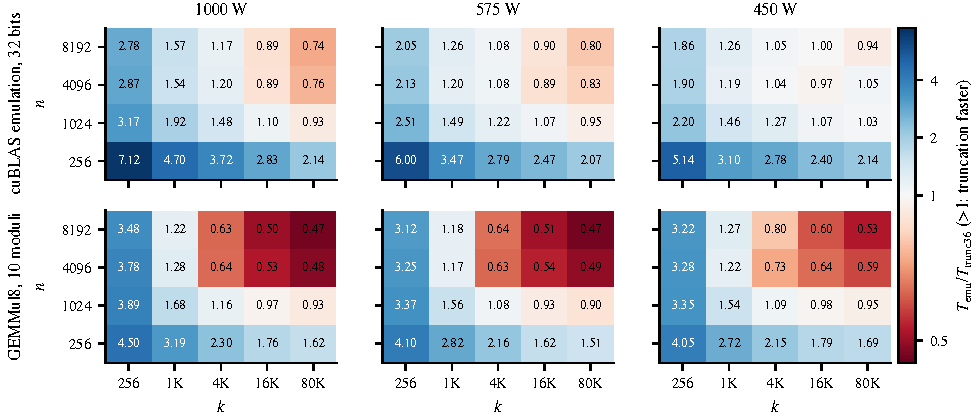
\includegraphics[width=\textwidth]{figs/crossover.pdf}
\caption{GH200: time of INT8 emulation relative to truncation to 36 bits, $T_\mathrm{emu}/T_\mathrm{trunc36}$
($m=8192$; blue: truncation faster). Top: cuBLAS emulation with 32 bits (error comparable to truncation,
$\approx10^{-11}$); bottom: GEMMul8 with 10 moduli (about ten times larger error, $\approx10^{-10}$); columns: module
caps. Means of two rounds.}\label{fig:crossover}
\end{figure*}

\textbf{A shape sweep and a predictive model (GH200).} We fixed $m=8192$ and swept $n\in\{256,1024,4096,8192\}$ and
$k\in\{256,1024,4096,16384,81920\}$ at 1000, 575 and 450\W, two rounds each (480 records; Fig.~\ref{fig:crossover}).
Truncation to 36 bits beat native in all 60 shape--cap combinations (3.8--11.9\pct{} at 450\W, 3.6--5.9\pct{} at
575\W, 0.5--4.8\pct{} at 1000\W). cuBLAS emulation with 32 bits wins roughly when $n\ge4096$ and $k\ge16384$ (and at
$n=1024$, $k=81920$ at 1000 and 575\W) (at best 0.74$\times$ truncation time at 1000\W), and its winning region shrinks at
lower caps: 5 of 20 shapes at 1000 and 575\W, 2 at 450\W. Where the emulation itself is not power-bound, however, lower
caps favor it: at $n=8192$, $k=4096$ its time relative to truncation falls from 1.17 to 1.08 to 1.05 as the cap goes from
1000 to 575 to 450\W. The four values of $n$ were measured on different nodes: each ratio is paired on one node, but
shape effects and node differences cannot be separated. GEMMul8 with 10 moduli needs only 0.47--0.80$\times$ the
truncation time when $n,k\ge4096$, at an order of magnitude larger error ($\approx10^{-10}$ versus $10^{-11}$), and is up
to 4.5$\times$ slower when $n$ or $k$ is small. Emulation's extra work is input splitting ($\propto mk+nk$) and output
accumulation ($\propto mn$); dividing by the $mnk$ multiply gives
\begin{equation}
T_\mathrm{emu}/T_\mathrm{trunc} = A + B\,(1/m + 1/n) + C/k,
\end{equation}
where $A$ is the ratio of per-flop speeds. Least-squares fits per cap (about 20 points for three parameters, so $R^2$ is
only descriptive) reach $R^2=0.98$--0.99 for GEMMul8, versus 0.86--0.89 for a single effective size
$1/(1/m+1/n+1/k)$; cuBLAS emulation reaches only 0.88--0.89. On the two held-out valinomycin shapes the model picks the
winner in 8 of 8 cases, all far from the crossover, so this is a loose test; the model is an empirical description of
these measurements.

\begin{figure*}[t]
\centering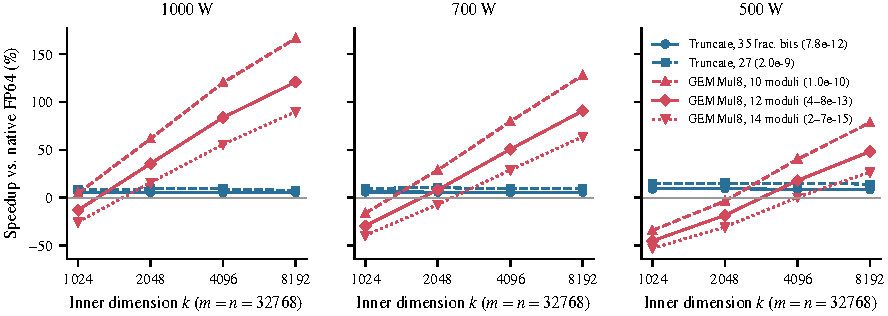
\includegraphics[width=\textwidth]{figs/mi350_crossover.pdf}
\caption{MI350X: speedup over native FP64 of truncation (round to nearest) and GEMMul8 for $m=n=32768$ as a function of
the inner dimension $k$, at three package caps (8 GPUs $\times$ ABBA, node n02). Relative errors in the legend. A tighter
cap lowers every emulation curve and raises every truncation curve.}\label{fig:mi350xover}
\end{figure*}

\textbf{MI350X: the cap moves the crossover.} On MI350X we compared truncation (35 and 27 bits, round to nearest) with
GEMMul8 3.2.0 (8--14 moduli) for $m=n=32768$ and $k=1024$--8192 at 1000, 700 and 500\W{} (Fig.~\ref{fig:mi350xover}).
Truncation to 35 bits ($\ee{7.8}{-12}$) is 5.1--5.5\pct{} faster than native at 1000\W{} and 8.3--9.3\pct{} at 500\W{}
for every $k$. GEMMul8 with 12 moduli ($\ee{4}{-13}$--$\ee{8}{-13}$, more accurate than 35 bits) is 13\pct{} slower than
native at $k=1024$ but 36, 84 and 121\pct{} faster at $k=2048$, 4096 and 8192 at 1000\W. At 500\W{} those gains fall
to $-45$, $-18$, +18 and +48\pct. The crossover thus moves with the cap: at $k=2048$ emulation wins at 1000 and 700\W{}
and truncation at 500\W, and at $k=1024$ truncation wins everywhere. The direction is the same as GEMMul8's on GH200
(Table~\ref{tab:methods}) and follows from power: GEMMul8 draws the full limit, and the extra integer work it does per
useful FP64 operation is paid for with clock when power is the constraint, whereas truncation removes work from the
power budget. The ratio of INT8 to FP64 throughput sets where the crossover lies; the cap sets which way it moves.

\begin{table}[t]
\caption{GH200: square GEMM ($32768{\times}32768{\times}2048$) in TFLOP/s by cap on one node, native FP64 first and the
other methods ordered by relative error.}\label{tab:methods}
\centering\footnotesize\setlength{\tabcolsep}{4pt}
\begin{tabular}{@{}lrrr@{}}
\toprule
Method (error) & 1000\W & 575\W & 450\W \\
\midrule
FP64 native & 59.2 & 43.2 & 35.8 \\
Trunc., 36 bits ($\ee{1.0}{-11}$) & 61.8 & 45.5 & 38.6 \\
GEMMul8, 10 moduli ($\ee{1.0}{-10}$) & 70.8 & 51.4 & 34.7 \\
GEMMul8, 9 moduli ($\ee{1.6}{-9}$) & 78.2 & 56.6 & 38.2 \\
cuBLAS emu., 28 bits ($\ee{2.3}{-9}$) & 67.8 & 55.2 & 47.5 \\
Trunc., 28 bits ($\ee{2.6}{-9}$) & 63.2 & 46.6 & 39.6 \\
FP32 SGEMM ($\ee{8.1}{-7}$) & 51.2 & 40.4 & 34.6 \\
3xTF32 ($\ee{4.8}{-6}$) & 96.6 & 72.0 & 56.4 \\
\bottomrule
\end{tabular}
\end{table}

\textbf{The power of the emulation itself changes the winner.} On GH200, GEMMul8 draws about 970\W{} at a 1000\W{} cap and at
450\W{} its clock drops to 650--720\,MHz, where truncation becomes faster; cuBLAS fixed-point emulation with 28 bits draws only
about 706\W{} at 1000\W{} and gains relative ground at lower caps on the square shape (Table~\ref{tab:methods}).
Which way a tighter cap tips the balance thus depends on how much power the emulation itself draws.

\textbf{Applications: memory and warm-up.} In DF-MP2 on MI350X ($k=5477$), GEMMul8 with 12 moduli is 34--67\pct{}
faster than native and beats truncation at every cap (Table~\ref{tab:mp2}), its lead again shrinking as the cap tightens.
Two costs appear only in applications. First, each new GEMM shape costs GEMMul8 a large one-time setup: DF-MP2 forms
226 shapes of growing $n$, and the first pass through them takes 142\,s instead of 13\,s (the native contraction takes
22\,s; pre-allocating the workspace does not help). Programs that call many distinct shapes once lose; the times in
Table~\ref{tab:mp2} exclude this warm-up. Second, emulation needs workspace. In HPL on MI350X the matrix of our best
native configuration ($N=540672$) occupies about 292\,GB per GPU, and GEMMul8's 15\,GB workspace no longer fits, so every
emulated run aborts; with 12 moduli even $N=491520$ does not fit. HPL's score grows with $N$, so emulation must give
up problem size before it can start. On the configuration used for GEMMul8's best MI350X result ($N=491520$, NB 4096,
$4\times2$), 10 moduli pass the residual check (1.79) \pending{HPL three-way comparison: native vs 36 bits vs
GEMMul8 10/12 moduli at $N=458752$ and 491520, four caps (jobs 49, 54)}.

\subsection{FP32 and 3xTF32: Accumulation, Not Range (GH200)}\label{sec:fp32}

3xTF32 (our own implementation, in the shim and in a benchmark script, not the CUTLASS one) is the fastest method in
Table~\ref{tab:methods} but has only FP32-level accuracy, and its error grows with the inner dimension: on $4096{\times}4096$ it is $\ee{6.4}{-7}$, $\ee{4.8}{-6}$ and $\ee{3.8}{-5}$ at $k=256$, 2048 and
16384, whereas FP32 SGEMM grows as $\sqrt{k}$ ($\ee{2.9}{-7}$, $\ee{8.1}{-7}$, $\ee{2.3}{-6}$) and FP64 truncation
is independent of $k$. The measured log slope of about one (7.5--7.9$\times$ per 8$\times$ in $k$) points to a
systematic error in TF32 tensor-core accumulation rather than random rounding, consistent with the round-toward-zero
accumulation Fasi et al.\ found on V100, T4 and A100~\cite{Fasi2021} (bit-accurate Hopper models:~\cite{Khattak2025}).
At $k=2048$ its error is 18 times that of FP64 rounded to nearest at 20 bits ($\ee{2.6}{-7}$) and 7 times that of
FP64 truncated to 20 bits ($\ee{6.7}{-7}$).

Quantum ESPRESSO's operands fit in FP32's range, so we replaced every FP64 and complex FP64 GEMM with single
precision through the shim (inputs to FP32; 3xTF32 additionally splits into big and small parts multiplied three
times on TF32 tensor cores; $C$ combined in FP64). On the gold surface at 450\W{} (2 interleaved runs each), FP32
aborts at SCF iteration 26 and 3xTF32 and TF32 at iteration 2 when the Davidson bands fail to converge, and the
integrated charge drifts from 1232 electrons (FP32 $+0.012$, 3xTF32 $+0.074$); FP64 rounded to 24 and 20 bits
differs from native by $\ee{8.1}{-6}$ and $\ee{5.5}{-5}$\Ry{} and converges in 28 iterations. Si\,1000 at 550\W{}
behaves the same: FP32 aborts at iteration 14 and 3xTF32 at 9, with 4000.18 and 4001.52 electrons instead of 4000.
The difference is accumulation: truncated FP64 still accumulates in FP64, while Quantum ESPRESSO's inner dimension
is the number of plane waves (95386 on the gold surface plus a real GEMM with $k=4.3{\times}10^{6}$; 375286 for
Si\,1000), where 3xTF32 already errs by $\ee{5.6}{-5}$ to $\ee{2.2}{-4}$, the same order as plain TF32. FP32 GEMM on
Hopper is also slower than FP64 tensor cores (on the gold surface about 1.5$\times$ per SCF iteration, estimated).
Replacing every GEMM with single precision thus fails for this long-inner-product solver even though the range fits;
mixed precision that uses FP32 only in selected steps, as Woo et al.\ do~\cite{Woo2023}, is a different matter. FP64
truncation is the reduced-precision choice here that leaves the algorithm unchanged.

\subsection{Exponent Span Limits Format Changes}\label{sec:span}

Truncation keeps every element's 11-bit exponent and changes only its mantissa; format changes must handle the
exponent. Per-tensor scaled formats (FP32, FP8) need the whole tensor inside the format's range, and Ozaki-type INT8
emulation slices each row (column) relative to its maximum, so with $k$ kept bits elements more than $2^{-k}$ below
the row maximum are lost. The exponent span of the data therefore limits format changes, whereas truncation is
unaffected.

\begin{figure}[t]
\centering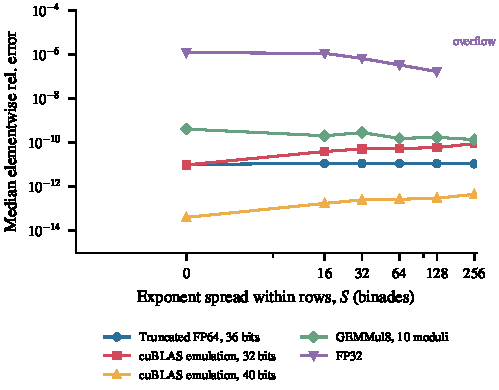
\includegraphics[width=\columnwidth]{figs/spread_error.pdf}
\caption{GH200, synthetic exponent spread: elements of $8192{\times}8192{\times}16384$ operands have exponents uniform over
$S$ binades within each row (1000\W).}\label{fig:spread}
\end{figure}

\textbf{Synthetic data.} On GH200, on $8192{\times}8192{\times}16384$, a shape where emulation is faster at narrow spans, we
draw element exponents uniformly over $S$ binades (1000/575\W, two rounds; Fig.~\ref{fig:spread}). Truncation to 36
bits keeps a median elementwise error of 1.0--1.1$\times10^{-11}$ and a speedup of 4.4--6.3\pct. cuBLAS emulation with
a fixed 32 bits degrades by 4--9$\times$ in median and 5--19$\times$ at p99 ($S=16$--256), the equivalent of 2--3
fewer bits, which costs a whole extra 8-bit slice to recover. Its dynamic mode, which targets FP64-equivalent
accuracy, raises the bit count from 58 to 301 and falls back to native FP64 beyond its maximum, but with the extra
work of determining the span it takes 1.6--2.6$\times$ the truncation time (2.6$\times$ at $S=16$); FP32 overflows
at $S=256$. GEMMul8 is barely affected on uniformly spread data. If the spread is only between rows (one scale per
row), emulation is unaffected while FP32 still overflows. \pending{MI350X: the same sweep with GEMMul8 10/12/14
moduli and truncation, $S=0$--64 per element and per row (job 53)}.

\begin{table}[t]
\caption{GH200, real data (1000\W): flop-weighted fraction of nonzeros more than $2^{-32}$ below their row maximum, and the
total-energy error of each method. The ``Nearest'' rows keep 36 or 32 bits with round-to-nearest; cuBLAS emulation
with 36 and 32 bits uses five slices, with 40 bits six; auto: its automatic mode (at most 79 bits). The Au\,112
fraction comes from a two-iteration benchmark input, its errors from the fully converged input.}\label{tab:span}
\centering\footnotesize\setlength{\tabcolsep}{4pt}
\begin{tabular}{@{}llll@{}}
\toprule
& Valinomycin & QE Si\,1000 & QE Au\,112 \\
\midrule
Below $2^{-32}$ & 24--44\pct & 0.24--0.54\pct & 0.008--0.02\pct \\
Nearest, 36 bits & $\ee{9.6}{-7}$\Eh & 0\Ry & 0\Ry \\
Nearest, 32 bits & $\ee{1.2}{-5}$\Eh & 0\Ry & $\ee{4}{-8}$\Ry \\
cuBLAS emu., 36/32 & $\mathbf{\ee{5.25}{-2}}$\,\textbf{E}$_\mathbf{h}$ & $\ee{6}{-8}$\Ry & $\ee{5}{-8}$\Ry \\
cuBLAS emu., 40 & $\ee{8.4}{-8}$\Eh & --- & --- \\
cuBLAS emu., auto & $\ee{4}{-9}$\Eh & --- & --- \\
GEMMul8, 10 moduli & diverges & out of memory & $\ee{3.7}{-7}$\Ry \\
\bottomrule
\end{tabular}
\end{table}

\textbf{Real data.} The shim samples 256 rows of op($A$) and 256 columns of op($B$) per GEMM and records the fraction
of nonzeros more than $2^{-32}$ below their row maximum, weighted by flops (validated against theory on synthetic
data). In Gaussian-basis DFT the atomic-orbital values on the grid decay exponentially with distance, and in the worst
shape 87\pct{} of elements are more than $2^{-32}$ below their row maximum. There, fixed 36-bit cuBLAS emulation
(five slices, like 32 bits) lets the SCF converge normally in 12 iterations to a total energy that is off by
52.5\,mE$_\mathrm{h}$ ($\approx$33\,kcal/mol), and GEMMul8 diverges; rounding to the same 36 bits errs by
$\ee{9.6}{-7}$\Eh{} (Table~\ref{tab:span}). What fails is the user-fixed bit count. With 40 bits (six slices) the
emulation is correct ($\ee{8}{-8}$\Eh) but takes about 1.5$\times$ the time of truncation to 36 bits, and
cuBLAS's automatic mode, capped at 79 bits, is correct too ($\ee{4}{-9}$\Eh): 89\pct{} of the flops would need 80 or
more bits and fall back to native FP64, the rest is emulated with 72--79 bits, and the run takes 2.1$\times$ the
native time. On wide-span data emulation is therefore not impossible, but not worthwhile. HPL sits at the other
extreme: only $\ee{2.7}{-6}$ of its flop-weighted elements are more than $2^{-32}$ below their row maximum, and fixed
36-bit emulation passes the residual check (0.197, against 0.057 for HPL's own rounding to 36 bits) but runs at
0.65$\times$ native speed on one GPU ($N=81920$; the automatic mode keeps the native residual level,
$\ee{1.9}{-6}$ against $\ee{1.7}{-6}$, at 0.35$\times$). On Quantum ESPRESSO, with narrow
per-row spans, fixed 36-bit emulation errs by only 5--$\ee{6}{-8}$\Ry. Uniform synthetic spreads understate the
problem, since in real data many elements of a row lie far below its maximum. A wide per-row span, which the shim measures cheaply beforehand (Fig.~\ref{fig:map}), is thus a risk indicator: a
necessary but not sufficient condition for failure, and tile-level mixed precision can also handle such data
(Section~\ref{sec:gp}). DF-MP2 (Section~\ref{sec:mp2}) sits at the narrow end, where FP32 works and GEMMul8 on MI350X is
accurate.

\begin{figure}[t]
\centering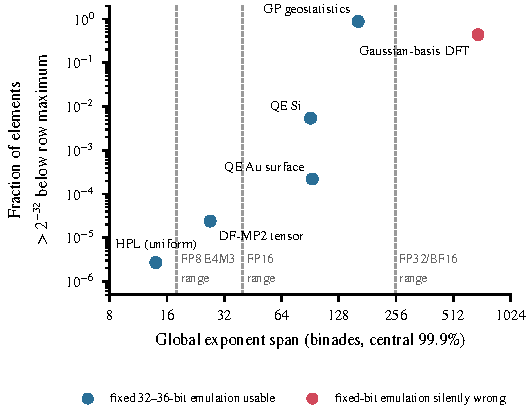
\includegraphics[width=\columnwidth]{figs/range_map.pdf}
\caption{GH200: global exponent span (central 99.9\pct) against the flop-weighted fraction of elements more than $2^{-32}$
below their row maximum, with the measured outcome of fixed 32--36-bit cuBLAS emulation (e.g., HPL: residual 0.197,
passes; Gaussian-basis DFT: 52.5\,mE$_\mathrm{h}$ error; Gaussian process: global span 162, estimate unchanged). All
points are measured; coordinates and their sources are listed in
\texttt{gh200/results/range\_map\_points.csv}.}\label{fig:map}
\end{figure}

\textbf{Wide range, partly power-bound DFT.} These DFT runs draw only 650--690\W{} at 1000\W, but are power-bound
below that. For valinomycin (grid level 6) at 550 and 450\W, rounding to 36 bits through the shim is 3.3--3.5\pct{}
faster than the copy baseline with 2--3\pct{} less energy and an error of $\ee{9.5}{-7}$\Eh; emulation must keep 40
bits to stay correct, which is then about ten times more accurate ($\ee{8.4}{-8}$\Eh) but takes 1.48--1.53$\times$
the baseline time (two rounds each).

\subsection{Wide Range and Power-Bound: Gaussian-Process Geostatistics}\label{sec:gp}

Maximum-likelihood estimation of a Gaussian process in geostatistics factors an $n{\times}n$ Matérn covariance matrix
by Cholesky at every likelihood evaluation. As in HPL, almost all work is FP64 matrix multiplication, but the
covariance decays exponentially with distance. We implemented an ExaGeoStat-like kernel, in CUDA with cuBLAS on GH200
and in HIP with rocBLAS/rocSOLVER on MI350X: $n=80000$ random 2-D locations, Matérn-3/2 covariance (nugget $10^{-4}$),
blocked Cholesky ($n_b=1024$, trailing updates by one FP64 DGEMM per panel), and the log-likelihood at six range
parameters (0.02--0.08). Each panel $L_{21}$ keeps $k$ bits before the trailing update, in one fused pass that walks
the panel in memory order (an earlier version with two separate, uncoalesced passes left 28 bits at 5.2--5.7\pct{} under
caps on GH200, so the reduction itself must be cheap). On GH200 we compare with cuBLAS emulation and FP32 (1000/700/500\W,
six interleaved rounds from two jobs on the same node); on MI350X each of the 8 GPUs runs the variants interleaved
(16 pairs per cap). Native draws 953--970\W{} of module power at 1000\W{} on GH200 and is capped 91--94\pct{} of the
time; on MI350X it draws 924\W{} per GPU and is held at the limit 86\pct{} of the time. The sampled panel rows span 162
binades (central 99.9\pct), and 88\pct{} of the panels' nonzeros are more than $2^{-32}$ below their row maximum.

\begin{table}[t]
\caption{Gaussian-process likelihood ($n=80000$, six range parameters): largest log-likelihood deviation from
native and speed relative to native (mean $\pm$ 95\pct{} $t$ interval; GH200: 6 rounds; MI350X: 16 pairs; truncation
rounds to nearest). The log-likelihoods are 1.2--1.7$\times10^5$.}\label{tab:gp}
\centering\footnotesize\setlength{\tabcolsep}{2.5pt}
\begin{tabular}{@{}lllll@{}}
\toprule
 & Trunc.\ 36 & Trunc.\ 28 & Emulation & FP32 \\
\midrule
\multicolumn{5}{@{}l}{\emph{GH200} (emulation: cuBLAS, 36 bits)} \\
$\max|\Delta\ell|$ & $\ee{2.4}{-5}$ & $\ee{7.2}{-4}$ & $\ee{2.2}{-3}$ & 87 \\
1000\W & $+3.0\pm0.3\pct$ & $+3.8\pm0.4\pct$ & $-41\pct$ & $-8.2\pct$ \\
700\W & $+5.0\pm0.1\pct$ & $+7.9\pm0.2\pct$ & $-31\pct$ & $+3.2\pct$ \\
500\W & $+4.8\pm0.1\pct$ & $+7.5\pm0.1\pct$ & $-21\pct$ & $+3.9\pct$ \\
\multicolumn{5}{@{}l}{\emph{MI350X} (emulation: GEMMul8)} \\
$\max|\Delta\ell|$ & $\ee{1.9}{-5}$ & $\ee{5.3}{-3}$ & \pending{} & --- \\
1000\W & $+4.0\pm0.2\pct$ & $+7.6\pm0.2\pct$ & \pending{} & --- \\
800\W & $+3.9\pm0.4\pct$ & $+6.1\pm0.7\pct$ & \pending{} & --- \\
650\W & $+5.4\pm0.7\pct$ & $+7.9\pm1.2\pct$ & \pending{} & --- \\
500\W & $+6.7\pm0.4\pct$ & $+10.9\pm0.6\pct$ & \pending{} & --- \\
\bottomrule
\end{tabular}
\end{table}

A deviation of $\ee{7.2}{-4}$ (GH200) or $\ee{5.3}{-3}$ (MI350X, different random locations) at 28 bits, a relative
$\ee{3}{-8}$--$\ee{4.5}{-8}$, is far below what matters for estimation (Table~\ref{tab:gp}). On GH200 at 1000\W, where
this native factorization is capped 91--94\pct{} of the time, 28 bits is 3.8\pct{} faster (36 bits 3.0\pct), but the
1000\W{} gain depends on the setting: with the Morton ordering used below ($n=60000$), where native is capped in only
19--54\pct{} of the samples, 28 bits gains +0.0/+0.1\pct, and the maximum-likelihood fit below gains 1.8--2.3\pct. On
MI350X the default limit binds, and 28 bits is 7.6\pct{} faster at 1000\W{} and 10.9\pct{} at 500\W, with 5.7--9.8\pct{}
less energy. FP32's deviation makes it unusable for estimation; it may stem from the conditioning of the covariance, which
worsens with $n$ (at $n=8000$ FP32 still finds the same estimate). cuBLAS emulation on GH200 is less accurate than 28-bit
truncation and slower, partly because the trailing update's inner dimension equals the block size, 1024, a shape that
already favors truncation in the crossover model (Section~\ref{sec:crossover}) and in the MI350X sweep, where GEMMul8 loses
to truncation at $k=1024$ under every cap. The per-row span is wider than in the DFT case, yet emulation does not go
wrong, only loses accuracy: a wide per-row span is necessary but not sufficient for emulation failure, which also depends
on how much the dropped small elements contribute.

\textbf{A one-parameter maximum-likelihood fit (GH200).} To check that the estimate itself is unchanged, we fitted the range
parameter with variance and smoothness fixed: golden-section search over its logarithm, 17 likelihood evaluations
per variant ($n=60000$; 1000 and 700\W; two interleaved rounds). Truncation to 36 and 28 bits and cuBLAS emulation
return the native estimate
$\hat\theta=0.05007952$ in every printed digit, with maximized log-likelihoods within $\ee{4.8}{-6}$ (36 bits) and
$\ee{2.3}{-4}$ (28 bits) of native; FP32 moves $\hat\theta$ by 0.49\pct{} and loses 0.72 in log-likelihood. At
700\W{} the fit is 7.1--7.3\pct{} faster with 28 bits
and 4.8--4.9\pct{} faster with 36 bits, using 6.6--6.8\pct{} and 4.5--4.8\pct{} less energy; at 1000\W{} it is
1.8--2.3\pct{} and 1.6--2.2\pct{} faster with 9.1--9.9\pct{} and 3.5--5.6\pct{} less energy; cuBLAS emulation is
32--41\pct{} slower. Of the three whole-matrix choices we tested (FP32, 36-bit cuBLAS emulation and truncation), only
truncation is both fast and accurate on this wide-range, power-bound workload.

\textbf{Composing with tile mixed precision (GH200).} The mixed-precision Cholesky factorizations of the ExaGeoStat line change
the format of whole tiles instead (Section~\ref{sec:related}). To see whether truncation still helps there, we ordered
the locations along a Morton curve and added such a variant to our kernel: in the trailing update, tiles below each
column's FP64 extent, chosen by the tile-norm rule with a required accuracy of $10^{-9}$ as in~\cite{Cao2023}, use FP16
inputs with FP32 accumulation on the tensor cores (52\pct{} of the tiles at range 0.02, 3\pct{} at 0.08). Over the six
ranges ($n=60000$, two ABBA rounds) it runs 1.60--1.63$\times$ faster than native FP64 at 1000, 700 and 500\W, with
log-likelihood deviations up to 0.043. Truncating its remaining FP64 tiles to 28 bits makes it another 1.9\pct{}
faster at 1000\W{} and 7.0\pct{} and 6.1\pct{} faster at 700 and 500\W, with an unchanged deviation, so truncation
composes with format changes rather than competing with them. Zeroing the FP16 operands to 5 mantissa bits as well
added nothing.

\textbf{ExaGeoStat itself (GH200).} We also built ExaGeoStatCPP (StarPU and Chameleon tile Cholesky with cuBLAS~13.6; tile
size 1920) and ran its MLE ($N=60000$, six BOBYQA likelihood evaluations per run, data generated once natively and
read by every run) with the shim on its FP64 tile GEMMs. Matérn covariance generation runs on the CPU and takes about
9\,s per evaluation against 2.3\,s of GPU factorization at 1000\W, and the factorization is partly power-limited even
there (GPU power about 620--670\W{} on average, frequent power-cap events). Relative to a baseline that copies the operands without
truncating, the factorization is 3.0\pct{} (36 bits) and 4.0\pct{} (28 bits) faster at 1000\W, 5.0\pct{} and
8.0\pct{} at 600\W, and 5.6\pct{} and 9.4\pct{} at 450\W{} (means of two ABBA rounds; at 450\W{} the rounds differ
widely, +6.9 and +11.9\pct{} with 28 bits at 707 and 926\,MHz, because the CPU shares the module cap while generating
the covariance); with 28 bits the mean SM clock during factorization rises from 1913 to 1975\,MHz at 1000\W{} and
from 1166 to 1305\,MHz at 600\W. The log-likelihoods change by at most $\ee{1.2}{-10}$ and $\ee{9.8}{-8}$ relative.
The shim's own copy costs 7--9\pct, which leaves it 0.5--3.1\pct{} slower than unmodified ExaGeoStat, so the gain
needs an implementation inside the library. ExaGeoStatCPP's mixed-precision option (\texttt{-{}-computation=mixed}) is
only an enumeration value without an implementation, so we could not compare with its own mixed precision.

\subsection{Truncation Inside Emulation}\label{sec:synergy}

Truncation and emulation are not exclusive. GEMMul8 converts each FP64 row into integers; if the operands carry only
$k$ significant bits, the low-order integer slices are largely zero and the INT8 matrix engines toggle less, so under a cap
the emulation itself should run faster, at the accuracy of $k$-bit truncation. \pending{MI350X: GEMMul8 8/10/12 moduli
on operands truncated to 35 and 19 bits versus full operands, 1000/700/500\W{} (job 51)}.

%==================================================================================================
\section{AI Workloads: Training and Inference (GH200)}\label{sec:ai}

MLPerf Training measures time to target quality (eval loss $\le0.925$ on GovReport for Llama\,2 70B LoRA); a faster
step that needs more samples to converge loses.

\textbf{Training: truncating the FP8 base weights is a negative result.} We truncated only the frozen FP8 base weights
of Llama\,2 70B LoRA (once, after loading); activations, gradients, LoRA weights and updates and per-tensor scaling
follow~\cite{Micikevicius2022}. On 8 nodes with the same seed, native FP8 at 575\W{} reached the target after 3456
samples in 28.34\,min. Keeping 2 bits made each 384 samples only 0.9--1.2\pct{} faster but needed 4224 samples (22\pct{}
slower at 575\W, 19\pct{} at 800\W); 1 bit did not converge (it also lowers the largest representable E4M3 value
from 448 to 384, compressing the top weights by about 14\pct). The eval-loss curve shifts up by 0.006--0.008, while
the train-loss gap varies (with 2 bits $-0.031$ at the first logged step, then $+0.003$ to $+0.017$): truncation
weakens the base model at load time, and a rank-16 adapter does not compensate. A second seed (5678, 800\W) agrees: native 3072 samples in 22.74\,min,
2 bits 4224 samples in 31.56\,min (+39\pct). Across two seeds and four pairs (one at 575\W, three at 800\W), the first evaluation is always
0.008--0.010 higher and convergence takes 2--3 more evaluation intervals. Native convergence differs by one interval
between node sets (3072 versus 3456), so we read this only as evidence that FP8's 3 mantissa bits leave no room. The
rounding mode shows no consistent order (at 800\W{} truncation and stochastic rounding converge at 4224 samples,
nearest at 5376). Truncating only MLP layers needs 4224 samples, attention only 3840 (one interval, within node-set
noise, but attention is only about 18\pct{} of the linear weights); the first-evaluation gaps of $+0.0064$ (MLP) and
$+0.0028$ (attention) roughly add up to the $+0.0086$ of full truncation (their sum is 0.0092). A repeat of the
attention-only run gave nearly the
same first evaluation (0.9428 versus 0.9425) but converged one interval later (4224 versus 3840, missing the target by
$10^{-5}$ at 3840), so the first-evaluation gap, not the convergence point, is the robust metric.

\begin{table}[t]
\caption{WikiText-2 perplexity (sequence 2048) relative to BF16 for the linear layers' formats; FP8 uses real FP8
tensor-core GEMMs, and kept bits are rounded to nearest (ties to even).}\label{tab:llm}
\centering\footnotesize\setlength{\tabcolsep}{2.2pt}
\begin{tabular}{@{}lrrrrrr@{}}
\toprule
Format & L2-7B & L3.1-8B & Qw2.5-7B & Mis-7B & OPT-6.7B & L2-70B \\
\midrule
BF16, 4 b & +0.09 & +0.19 & +0.13 & +0.09 & +0.45 & +0.10 \\
BF16, 3 b & +0.44 & +1.02 & +0.65 & +0.41 & +2.00 & +0.51 \\
FP8 per tensor & +0.63 & +0.95 & +0.70 & +0.45 & +2.23 & +0.48 \\
FP8 per channel & +0.32 & +0.88 & +0.61 & +0.34 & +0.69 & +0.42 \\
FP8 p.c., 2 b & +3.2 & +6.5 & +4.0 & +2.5 & +7.0 & +3.4 \\
FP8, wts.\ 2 b & +1.9 & +4.0 & +2.6 & +1.3 & +2.8 & --- \\
\bottomrule
\end{tabular}
\\[2pt]{\scriptsize Values in percent. b: kept bits; L: Llama, Qw: Qwen, Mis: Mistral; p.c.: per channel; wts.: weights only.}
\end{table}

\textbf{Inference: FP8 has already taken most of the benefit.} BF16 rounded to nearest at 3 bits has as many mantissa
bits as FP8 E4M3 and matches its accuracy on six language models (Table~\ref{tab:llm}; with truncation, 4 bits are
needed for a similar GEMM error, 4.35\pct{} on uniform data). We then compared the two where FP8 is known to fail:
attention perplexity at 2k/8k context (BF16 3 bits +0.49/+1.06\pct, emulated FP8 attention +0.52/+1.08\pct), key
retrieval at 8k--32k context on Llama-3.1-8B (both 100\pct), BERT-large SQuAD (all formats above 99.9\pct{} of FP32
F1) and CogVideoX-2B video generation (PSNR against native 18--38\,dB for FP8 attention, 20--29\,dB for BF16 3 bits).
With proper scaling the two tie, and FP8 GEMMs are about 1.7--1.9$\times$ as fast (at 575\W, 1.67--1.72$\times$
BF16 with 3 bits and 1.80--1.87$\times$ native BF16). A naive FP8 attention that does not scale the softmax probabilities fails as sequences grow (74\pct{}
error at 4096 tokens), and on CogVideoX-2B (about 18k tokens) it changes the composition and adds noise (PSNR
10--12\,dB, SSIM 0.07--0.66) where BF16 with 3 bits keeps 20--21\,dB and SSIM 0.82--0.91. This is a range problem,
not a mantissa problem: the smallest positive E4M3 value, about $2^{-9}$, exceeds the mean attention probability over
18k tokens, while BF16 has 8 exponent bits; correct implementations already fix it inside FP8~\cite{Zhang2025}.

Without switching to 2:4 structured sparsity or INT4 weights, zeroing on top of FP8 is the remaining way to go faster
than FP8 on Hopper, which lacks FP4. On real layer-40 activations and weights of Llama2-70B
($8192{\times}57344{\times}8192$), keeping 2 bits on both sides is 4.4/3.2/5.0/8.2\pct{} faster at
1000/700/575/450\W, weights only 1.3--3.3\pct, but 70B perplexity rises by 3.4\pct. Per-layer sensitivity shows
q/k/v as least sensitive but a small share of the compute (with grouped-query attention, q is about 7.8\pct{} and k
and v about 1\pct{} each), and the MLP layers as most of the compute but more sensitive. FP8's
advantage comes mainly from halving the data path: at 575\W{} BF16 with 3 bits is only 8\pct{} faster than BF16,
while FP8 is 1.8$\times$. Power savings are limited too. Decode (64 tokens) is bandwidth-bound; at 1000\W{} zeroing
leaves its speed unchanged on uniform data, though on real Llama2-70B weights zeroed FP8 is still 2.6--3.0\pct{}
faster at the same clock. FP8 zeroed to 0 bits saves
104\W{} on uniform data but only 61\W{} on real Llama2-70B weights, and truncating weights to 2 or 0 bits saves only
1.5\pct{} or 5.5\pct{} of power at an accuracy cost. Below 575\W{} these savings turn into 2--16\pct{} speedups, and
prefill is power-bound even at 1000\W.

For weights and activations that directly set model quality and have no residual correction, zeroing turns directly
into quality loss, in contrast with solvers such as HPL-MxP and SCF that correct errors. For GPUs without FP8 tensor
cores, or pipelines that must stay in BF16, BF16 with 3--4 kept bits is a nearly lossless option; for FP8 deployments,
zeroing saves only 1.5--5.5\pct{} of power in memory-bound phases, at an accuracy cost.

%==================================================================================================
\section{Discussion}\label{sec:discussion}

\textbf{Where truncation pays.} Three conditions decide the gain: the GPU must be power-bound (or the saving shows
only as lower power), the truncated operands must flow directly and in volume into multipliers or data paths, and the
algorithm must tolerate the error, ideally by correcting it (refinement, self-consistency). The model of
Section~\ref{sec:model} makes the first quantitative: the equivalent saving is a fixed fraction $1/R-1$ of the dynamic
part of the cap, so a kernel's locked-clock energy ratio predicts its benefit under every cap. The second explains why
GEMM-dominated solvers (HPL, HPL-MxP, DF-MP2, the GP likelihood) gain 4--20\pct{} while N-body, MFEM, SW4 and LAMMPS gain
little. The third separates HPC solvers, which tolerate 20--36 bits, from AI weights, which have no residual correction
(Section~\ref{sec:ai}).

\textbf{The stock limit is a power cap.} On GH200 the gain at the default 1000\W{} module cap is mainly energy
(7.5--8.6\pct{} less per HPL solve) with 0.6--3.9\pct{} more speed. On MI350X the default 1000\W{} package limit binds for
FP64, BF16 and FP8 matrix work, for HPL, HPL-MxP, DF-MP2 and the GP likelihood alike, so truncation turns directly into
4.6--10\pct{} more speed at stock settings. As accelerators raise their throughput faster than their power envelope,
running at the limit becomes the default operating point rather than a datacenter policy, and the energy per operation,
including the share spent on toggling unneeded bits, becomes a first-order performance parameter.

\textbf{Benefit under a fixed power budget.} Under a fixed power budget, such as a rack limit, the equivalent power
saving becomes usable compute. At 8 GH200 nodes $\times$ 700\W, tuned HPL with the safe 36 bits rises from 346.2 to
362.9\,TFLOP/s on set A (+4.8\pct; set B +3.9\pct); native HPL would need about 768\W{} per node (774\W{} on set B),
about 0.5--0.6\,kW more for the cluster, to match. On one MI350X node at 800\W{} per GPU, the same 36 bits is worth
43--50\W{} per GPU, about 0.35--0.4\,kW per node. The cost is one bitwise operation per element, which can be fused
into the kernel that produces the operand, and no hardware. At 575\W{} the SM clocks of our 14 GH200 nodes differ by
17\pct{} (1129--1325\,MHz), and synchronous runs move at the pace of the slowest node, as earlier work found for CPUs
under power bounds~\cite{Rountree2012,Inadomi2015}; zeroing and variation-aware caps are complementary.

\textbf{Truncation and emulation.} INT8 emulation of FP64 is the stronger lever where its throughput advantage is
large and it can amortize its fixed costs: on MI350X it is up to 2.2$\times$ native for large $k$ and 1.7$\times$ in DF-MP2.
Truncation remains the better choice where emulation cannot amortize (small $k$ or $n$, many distinct shapes), where the
cap is tight, where memory is full, where per-row exponent spans are wide, outside matrix multiplication, and for BF16
and FP8, for which no emulation exists. Applied inside emulation it may reduce emulation's own power
(Section~\ref{sec:synergy}). A runtime that knows each call's shape, the cap and a cheap span estimate can choose per call.

\textbf{Benchmark rules.} The TOP500 Linpack rules require full 64-bit floating-point arithmetic and explicitly
exclude solving in lower precision with iterative refinement, and emulating floating point with integer
arithmetic~\cite{TOP500Linpack}; HPL on truncated operands does not meet the full-precision requirement either.
Since June 2025 the HPL-MxP rules require at least 16-bit floating point and allow diagonally dominant
test matrices for testing only~\cite{HPLMxPRules}; BF16 keeping 3 bits is effectively a 12-bit format, and our test matrix
is not allowed for official runs. All HPL and HPL-MxP numbers here are therefore research results, not official
scores. MLPerf Inference closed division allows any mathematical quantization but forbids
pruning~\cite{MLPerfInfRules}; zeroing is the former. Whether MLPerf Training permits truncated weights depends on
each round's rules; in our results uniform truncation does not pay anyway. Scientific software has no such
restriction; the criterion is whether physical results stay within the required accuracy.

\textbf{A hardware counterexample.} An Altera patent states that zeroing low bits at the input of an FPGA
floating-point multiplier has ``barely any effect on reducing the amount of power'' because the compression tree
keeps switching~\cite{Altera2017}. This does not contradict our measurements: the patent is a qualitative statement
about a $27{\times}27$ fixed-point multiplier, whereas on a GPU the truncated bits also travel through registers,
operand buses and memory, whose toggles disappear as well. Table~\ref{tab:fill2} supports this: a pure memory copy
saves 9--18\pct{} of power without any multiplication, mostly from the absence of toggles, while in the multipliers of
both GPUs zeros still save more than ones (Section~\ref{sec:why}).

\textbf{Limitations and threats to validity.} (i)~Two platforms, one generation each. The mechanism, the model and the
direction of the cap effect on the emulation crossover hold on both, but the size of the gain depends on each part's
power management, its INT8-to-FP64 ratio and its cooling, and other generations may differ. The MI350X results come from
two nodes of one system, each with 8 GPUs, and the HPL and HPL-MxP numbers are single-node (8-GPU) runs, not multi-node.
(ii)~The HPL residual is a deterministic but chaotic function of $N$, and the safe bit count is platform-dependent
(28 bits passes at three of four sizes on GH200 and at none on MI350X), so operating points (36 bits for HPL, 3 for
HPL-MxP) were validated at several sizes on each platform. (iii)~HPL-MxP used a diagonally dominant test matrix
(diagonal equal to the row's off-diagonal magnitude sum) with approximate diagonal factorization, which the rules allow
only for testing~\cite{HPLMxPRules}; its stability at 3 kept bits may be a property of this matrix. (iv)~Each scientific
code was tested on one or two input systems; forces, geometry optimization and larger systems are not covered, and on
MI350X DF-MP2 uses our own contraction of PySCF's tensor rather than GPU4PySCF. (v)~The GH200 shim costs 3--9\pct{} for
copies depending on the application, so shim results are always compared with a baseline taking the same copy path;
in-program zeroing has no such cost. (vi)~GH200 nodes differ by 13--17\pct{} at equal power and the GPUs of one MI350X
node by up to 30\pct{} in clock in synchronous HPL-MxP, so all comparisons are paired on the same nodes or GPUs by ABBA
order or by seed; intervals treat pairs within a job or node as independent, and moving HPL to a second GH200 node set
lowered its gain at 600--800\W{} by 0.5--0.9 points, more than pairs within a job differ, while the two MI350X nodes
agree within 2 points. (vii)~The default caps are also the highest, not uncapped states; the limiters' time scales are
unknown; and GH200 caps below 450\W{} lie outside the datasheet range~\cite{NVIDIAGH200}. (viii)~Cooling changes
conclusions: on GH200 at low fan speed the GPU hits its thermal limit first and at full fan speed native HPL-MxP at
1000\W{} trips the hardware power brake; on MI350X, chassis fans reacting to the previous run biased one multi-variant
comparison (Section~\ref{sec:setup}). The GEMM sweeps, the GP and the DF-MP2 runs use multi-variant orders; they were
replicated on a second node (GEMM) or run as ABBA within one process, which cancels linear drift but not this nonlinear
effect. (ix)~The GH200 cluster is shared and another user's tool reset caps at least twice, so every window checks the
cap in effect. (x)~Power comes from the devices' own sensors, not an external meter. On MI350X energy comes from a
hardware accumulator rather than sampled power, but it is still the device's own estimate. GH200 module power also
includes the Grace CPU and memory; all energy figures are relative values on one path per platform. (xi)~The
clock reduction we attribute to circuit-level clock stretching on MI350X is an inference: no available counter reports
it. The model's residual errors grow where the truncated program runs at clocks the native program never reaches.
(xii)~Not all of the Quantum ESPRESSO gain is a power effect: on the gold surface about half comes from fewer Davidson
iterations, for reasons not yet identified. (xiii)~The real-data emulation comparisons on Quantum ESPRESSO ran once per
setting, and GEMMul8 ran out of GPU memory on two GH200 applications and on MI350X HPL at the largest $N$. (xiv)~The
Gaussian-process results come from our ExaGeoStat-like kernel on synthetic data, and its mixed-precision variant is a
simplified re-implementation; ExaGeoStat itself was measured only through the shim, whose copy cost offsets the gain.

%==================================================================================================
\begin{table*}[t]
\caption{Where each mechanism and experiment lives in the repository.}\label{tab:artifact}
\centering\footnotesize\setlength{\tabcolsep}{4pt}
\begin{tabular}{@{}p{0.4\textwidth}p{0.56\textwidth}@{}}
\toprule
Path & Content \\
\midrule
\path{gh200/bench/}, \path{mi350/bench/} & mantissa GEMM microbenchmarks (cuBLAS; rocBLAS/hipBLASLt with GEMMul8 hook, transposes, exponent spread) and non-GEMM FP64 kernels \\
\path{gh200/shim/mantshim.cu} & cuBLAS interposer: rounding modes, cuBLAS emulation (fixed and automatic, bit-count log), FP32/3xTF32 replacement, exponent-span statistics \\
\path{rocHPL/src/blas/HPL_quantize_device.cpp} & HPL operand rounding (\path{HPL_QUANT_*_BITS}); the AMD build is branch \path{feat/adaptive-mixed-storage} \\
\path{rocHPL-MxP/src_mi350/hplmxp.h} & HPL-MxP zeroing on BF16 write-back (compile-time \path{MANT_BITS}), same source for both platforms \\
\path{apps/q-e/KS_Solvers/Davidson/} & in-program truncation and the tolerance-driven rule (\path{QE_MANT_ADAPT}) \\
\path{apps/pyscf-inputs/mp2_variants.py}, \path{mi350/apps/mp2_prep.py}, \path{mi350/apps/dfmp2.hip} & DF-MP2 variants on GH200; tensor preparation and HIP contraction on MI350X \\
\path{apps/geostat/gp_mle.py}, \path{mi350/apps/gp_chol.hip} & Gaussian-process likelihood and MLE (CUDA/cupy and HIP) \\
\path{apps/patches/} & MFEM, SW4, LAMMPS and ExaGeoStatCPP changes \\
\path{gh200/slurm/}, \path{mi350/scripts/}, \path{mi350/tools/} & job scripts (cap sweeps with ABBA or pairwise ABBA order); MI350X power-cap tool and amdsmi sampler with energy accumulator \\
\path{gh200/analysis/}, \path{mi350/analysis/} & summaries, $\Delta W$, intervals, crossover fit, power model (\path{power_model.py}), figures \\
\path{gh200/results/}, \path{mi350/results/} & summarized CSV files behind every table and figure \\
\bottomrule
\end{tabular}
\end{table*}

\section{Conclusion}\label{sec:conclusion}

On production GPUs of two vendors, truncating unused mantissa bits in software buys real performance for real HPC
applications under power limits while their physical results stay within each code's own criterion. The mechanism is the
same on both: bits that stop toggling, in matrix engines, vector units and data paths, account for most of the saved
energy, and a two-parameter model built on it predicts the gain under any cap from one calibration. What differs is the
operating point: GH200 gains mainly under lowered caps, whereas MI350X is power-bound at its stock limit, so FP64 HPL
keeping 36 bits is 4.6--5.1\pct{} faster, HPL-MxP keeping 3 bits 4.9--5.1\pct{} (7.6 to 8.0\,PFLOP/s per node), a
Gaussian-process likelihood 7.6\pct{} and DF-MP2 10.2\pct{} faster at default settings, and 6--20\pct{} at 500\W.
Microbenchmarks give upper bounds (up to 65\pct{} for FP64 with 0 kept bits at 400\W), not application operating
points. The scope is equally clear. INT8 emulation of FP64 is faster for long inner dimensions at generous caps, by up
to 2.2$\times$ on MI350X, but a tighter cap moves the crossover toward truncation on both platforms, emulation needs
workspace that limits problem size and warm-up that penalizes many distinct shapes, and on data with a wide per-row
exponent span fixed-width emulation can silently go wrong; replacing every GEMM with FP32 or 3xTF32 fails on long inner
products; kernels whose intermediates regrow full mantissas gain little; and for FP8 AI inference, further zeroing
trades accuracy for speed. Safe bit counts must be validated on the target platform, and measurements must control for
cooling feedback. Mantissa zeroing costs one bitwise operation per element, needs no hardware support, and complements
format changes. All HPL, HPL-MxP and MLPerf numbers here are research results, not official scores.

\section*{Data and Code Availability}
The mantissa shim, the in-program truncation of each application, the job scripts, the raw measurement logs, the
summarized CSV files and the scripts that draw every figure are in the project repository (branch
\path{mi350-study}). \path{gh200/analysis/paper_figures.py} and \path{mi350/analysis/paper_figures_mi350.py}
regenerate every figure of this paper from the CSV files in \path{gh200/results/} and \path{mi350/results/}.

\appendices
\section{Artifact Description}\label{app:artifact}

\textbf{Hardware and power control.} GH200: fourteen nodes, each with one NVIDIA GH200 480GB superchip (aarch64), 200\,Gb/s
InfiniBand, Slurm partition \path{compute}; module power caps are set with the cluster's \path{nv_power} tool only on
exclusively allocated nodes; fans were left at the operator's setting. MI350X: two nodes with 8 MI350X OAM GPUs each,
Slurm partition \path{gpu}; package power limits (PPT0) are set per GPU with \path{amd-smi set -o PPT0} and read back
from sysfs; clocks for the locked-clock experiments with \path{amd-smi set -L sclk max}. Every job restores the default
limit (and clock) on exit and records the cap in effect in each measurement window.

\textbf{Software.} GH200: NVHPC 26.5 (CUDA 13.2, cuBLAS 13.4, NCCL 2.29, HPC-X Open MPI 5), driver 615.71; ExaGeoStatCPP links
cuBLAS 13.6. HPL is a CUDA port of rocHPL (branch \path{feat/cuda-port}) and HPL-MxP the \path{perf/h200-mantissa}
branch of an HPL-MxP implementation~\cite{Dongarra2025}; Quantum ESPRESSO 7.6~\cite{Giannozzi2020}; GPU4PySCF
1.8.1~\cite{Wu2025,Li2025}; MFEM 4.10.1 (CUDA, partial assembly); SW4 (\path{raja} branch, commit 52b51c9, RAJA
2026.07.1); LAMMPS 22 Jul 2025 Update~6 (KOKKOS, CUDA); GEMMul8 3.5.1; MLPerf Training Llama\,2 70B LoRA with NVIDIA's
v5.0 implementation. MI350X: ROCm 7.2.3 (rocBLAS, hipBLASLt, rocSOLVER, RCCL), amdgpu 6.16.13, Open MPI 5.0.7 with UCX;
rocHPL branch \path{feat/adaptive-mixed-storage} (commit 37d0475), the same HPL-MxP source; GEMMul8 3.2.0 (commit
833e576); PySCF 2.14. Analysis uses Python with pandas, NumPy and Matplotlib.

\textbf{Code and data.} Table~\ref{tab:artifact} lists where each part lives; the experiment logs in \path{gh200/} and
\path{mi350/} record every job, including failed, cancelled and repeated ones, and every table and figure names its jobs
and result files there.

\textbf{Reproduction.} Each experiment is one job that sets caps only on its own nodes, waits for the GPUs to cool
before each run, interleaves variants in ABBA (or pairwise ABBA) order and writes power logs next to the program output;
an analysis script then joins run windows with the power logs. For example, the GH200 crossover sweep of
Section~\ref{sec:crossover} is \path{gh200/slurm/e1_gemm_tdp.sbatch} with the shapes, caps and methods passed as
environment variables, summarized by \path{gh200/analysis/crossover.py}; the MI350X sweeps are
\path{mi350/scripts/e1_gemm_tdp.sh} (GEMM, crossover, locked clocks via \path{e1b_fixedclk.sh}),
\path{hpl_tdp.sh} (HPL and HPL-MxP), \path{gp_tdp.sh} and \path{mp2_tdp.sh}, submitted through
\path{mi350/slurm/run.sbatch} and summarized by \path{mi350/analysis/e1_summary.py}, \path{hpl_summary.py},
\path{gp_summary.py} and \path{mp2_summary.py}; the model is \path{mi350/analysis/power_model.py}.

\bibliographystyle{IEEEtran}
\bibliography{refs}

\end{document}

